\documentclass[runningheads]{llncs}

\begin{document}

\title{Explicabilité additive et décorrélation structurelle dans les graphes complexes}
\titlerunning{Explicabilité et décorrélation dans les graphes}

\author{Guilhem DUPUY \\Encadré par Rémy CAZABET}
\authorrunning{G. DUPUY}

\institute{Université Claude Bernard Lyon 1, France}
%
\maketitle              % typeset the header of the contribution

% --- Début du bloc résumé ---
\addvspace{1.5em}
\begin{quotation}
\begin{small}
\noindent \textbf{Résumé.} La prédiction de liens dans les réseaux complexes est traditionnellement abordée comme une tâche purement prédictive. Ce travail propose de l'utiliser comme un instrument métrologique permettant de quantifier et d'interpréter la pertinence de différents paradigmes de l'état de l'art (topologiques, communautaires et géométriques) pour expliquer l'organisation d'un graphe. Nous développons un cadre d'explicabilité \textit{post-hoc} additive fondé sur le couplage d'un méta-classificateur non linéaire (\textit{XGBoost}) et de la théorie des jeux coopératifs via les valeurs de Shapley (SHAP). Ce modèle permet d'isoler les forces structurantes du réseau à l'échelle locale (la dyade) et globale (le graphe complet). 

Pour valider ce framework sur une source de vérité connue, nous introduisons un protocole de génération de graphes hybrides synthétiques géométrico-communautaires, corrigé des biais de filiation par un algorithme d'alignement numérique des variances théoriques. L'expérimentation met en évidence une limite conceptuelle majeure de la littérature : une forte colinéarité et redondance informationnelle entre les algorithmes de blocs (ex. Louvain) et les plongements d'espaces latents (ex. \textit{node2vec}), qui s'ajustent mutuellement sur leurs signaux respectifs, altérant l'explicabilité causale. 

Pour lever ce verrou, nous proposons deux méthodes originales d'inférence de caractéristiques décorrélées par débiaisage spatial : d'une part, une approche de détection de communautés intégrant un modèle nul gravitaire au cœur du calcul de modularité de Louvain, et d'autre part, une approche d'inférence d'\textit{embedding} ($\text{SiNEcustom}$) apprenant un plongement vectoriel sur la matrice des résidus du modèle nul. Validées statistiquement sur notre \textit{benchmark}, ces contributions démontrent l'efficacité de l'orthogonalisation pour isoler les facteurs d'influence au sein des structures complexes, ce qui favorise l'explicabilité.

\vspace{0.4cm}
\noindent \textbf{Mots-clés:} Prédiction de liens, Intelligence artificielle explicable (XAI), Valeurs de Shapley, Modèles en blocs stochastiques, Plongement de graphes, Modèles nuls, débiaisage.

\vspace{1.3cm} % Un peu d'espace entre les deux versions

\noindent \textbf{Abstract.} Link prediction in complex networks is traditionally approached as a purely predictive task. This work proposes to use it as a metrological instrument to quantify and interpret the relevance of various state-of-the-art paradigms (topological, community-based, and geometric) in explaining graph organization. We develop an additive \textit{post-hoc} explainability framework based on coupling a non-linear meta-classifier (\textit{XGBoost}) with cooperative game theory via Shapley values (SHAP). This model isolates the structuring forces of the network at both the local scale (the dyad) and the global scale (the full graph).

To validate this framework against a known ground truth, we introduce a generation protocol for synthetic hybrid geometric-community graphs, corrected for lineage bias using a numerical alignment algorithm for theoretical variances. The experimentation highlights a major conceptual limitation in the literature: a strong collinearity and informational redundancy between block algorithms (e.g., Louvain) and latent space embeddings (e.g., \textit{node2vec}), which mutually adjust to their respective signals, thereby impairing causal explainability.

To overcome this bottleneck, we propose two original methods for inferring decorrelated features through spatial debiasing: on the one hand, a community detection approach incorporating a gravity null model into the core of the Louvain modularity optimization, and on the other hand, an embedding inference approach ($\text{SiNEcustom}$) that learns a vector embedding on the residual matrix of the null model. Statistically validated on our \textit{benchmark}, these contributions demonstrate the effectiveness of orthogonalization in isolating factors of influence within complex structures, thereby enhancing explainability.

\vspace{0.4cm}
\noindent \textbf{Keywords:} Link prediction, Explainable artificial intelligence (XAI), Shapley values, Stochastic block models, Graph embedding, Null models, Debiasing.
\end{small}
\end{quotation}
\addvspace{4.5em} 

%%%%%%%%%%%%%%%%%%%%%%%%
%%% DEBUT DU RAPPORT %%%
%%%%%%%%%%%%%%%%%%%%%%%%

\section{Introduction}
\label{sec:introduction}

Ce rapport présente les travaux de recherche menés du 16 mars au 17 juillet 2026 dans le cadre de mon stage de fin d'études de Master 2 Informatique, spécialité Intelligence Artificielle, à l'Université Claude Bernard Lyon 1. Ce stage s'est déroulé au sein de l'équipe \textbf{DM2L} (Data Mining \& Machine Learning) du \textbf{LIRIS} (Laboratoire d'Informatique en Image et Systèmes d'Information), sous la direction de \textbf{Rémy Cazabet}, maître de conférences. 

L'équipe DM2L centre ses activités de recherche sur l'extraction et la découverte de connaissances à partir de données (Data Mining), via des approches  automatisées et semi-automatisées. Bien que ce stage se focalise sur l'extraction de données depuis des Graphes, leurs recherches s'appliquent également à d'autres représentations telles que les données spatio-temporelles, tenseurs, ensembles, ou encore au texte dans le cadre du Natural Language Processing. L'équipe est particulièrement active sur des thématiques au cœur de ce projet, dont le \textit{Graph Learning \& Mining} (graphes dynamiques, attribués, temporels) et l'intelligence artificielle explicable (\textit{XAI}). Son objectif fondamental est de proposer des contributions théoriques et algorithmiques qui permettent aux experts d'améliorer la qualité des connaissances qu'ils sont en capacité d'extraire de leurs données, ou d'en extraire de nouvelles.


\subsection{Contexte et Motivation Scientifique}
L'analyse de réseaux s'appuie en grande partie sur des modèles statistiques et d'apprentissage pour capturer les propriétés structurelles des graphes. Dans ce domaine, la \textbf{prédiction de liens} (\textit{link prediction}) est traditionnellement abordée comme une tâche prédictive visant à anticiper l'apparition d'arêtes futures ou manquantes. Cependant, dans le cadre de ce projet de recherche, la prédiction de liens n'est pas considérée comme une fin en soi, mais plutôt comme un \textbf{indicateur métrologique} : elle permet de mesurer à quel point une formalisation mathématique ou une structure observée (communautés, blocs, embeddings) explique fidèlement le graphe observé.

De nombreux modèles (Louvain\cite{louvain2008}, SBM\cite{sbm1983}, modèles d'espace latent\cite{deepwalk2014}\cite{node2vec2016}) excellent dans cette tâche, et il a été montré que les stacker permet d'atteindre d'excellentes performances\cite{01stackingLinkPred}, égalant même l'état de l'art.

Cependant, comprendre et quantifier précisément la contribution de chaque structure sous-jacente reste un défi majeur. Ce projet part de l'hypothèse que les graphes réels sont issus d'une pluralité de facteurs qui influencent en parallèle la création de lien, avec des interactions non linéaires complexes entre eux. Les méthodes actuelles d'explicabilité appliquées aux graphes fournissent principalement des explications locales sous forme de sous-graphes pondérés. L'interprétation cognitive de ces sous-graphes reste entièrement à la charge de l'utilisateur, ce qui limite leur transférabilité et leur rigueur opérationnelle.

\subsection{Objectifs du Stage}
Ce projet, par nature très exploratoire, vise à lever ce verrou en offrant de nouvelles pistes d'explication. 

La première est la conception d'une nouvelle méthode d'\textit{explicabilité multi-modèle additive}, conceptuellement inspirée de l'approche SHAP (\textit{SHapley Additive exPlanations}) issue de la théorie des jeux coopératifs \cite{lordShapleyOriginal_1953}. 

L'originalité de l'approche consiste à décomposer la probabilité de prédiction d'un lien non pas en fonction de variables de nœuds isolées, mais comme une \textbf{somme d'effets} provenant de différents modèles de graphes globaux préalablement ajustés sur le réseau d'intérêt. Nous considérons ainsi une approche multi-modèle combinant par exemple :
\begin{itemize}
    \item La structure topologique (centralité, degré, ...)
    \item Les structures de communautés (Louvain, SBM, ...) ;
    \item Les modèles d'espace latent (\textit{latent space models} tel que \textit{node2vec}) ;
\end{itemize}

Pour un graphe donné, l'objectif est de fournir \textbf{une explicabilité locale :} c'est à dire déterminer pour un couple de nœuds $(u, v)$ donné les facteurs explicatifs dominants (par exemple, l'appartenance à une même communauté ou la proximité latente). Et également \textbf{une explicabilité globale :} permettre, par sommation des explications locales, de caractériser la topologie et les forces structurantes du réseau dans son ensemble.

La seconde est l'exploration de méthodes d'inférence de métriques décorrélées entre elles, ou par rapport à une référence connue. Bien que le stacking d'un grand nombre de modèles permette d'atteindre d'excellentes performances, les modèles qui le composent capturent des informations très redondantes, ce qui en complexifie l'explicabilité. L'inférence de métriques décorrélées permettrait de résoudre ce problème en offrant une décomposition où chaque modèle ou métrique capture un facteur d'influence unique.
Ce stage propose 2 approches de ce type, permettant respectivement l'inférence de communautés de Louvain, et d'embeddings, décorrélés par rapport à la position (réelle ou inférée) de noeuds.

\subsection{Structure du Rapport}
Pour rendre compte de ces travaux, ce rapport est structuré comme suit :
La \textbf{partie 2} présente l'état de l'art des méthodes et modèles de prédiction de liens, des modèles structurels de graphes et des fondements théoriques de l'explicabilité additive.
Le \textbf{Chapitre 2} détaille la formalisation mathématique et l'architecture du modèle XAI multi-modèle développé durant ce stage.
Le \textbf{Chapitre 3} expose le protocole expérimental, les simulations sur réseaux synthétiques et réels, ainsi qu'une analyse critique des résultats obtenus.
Enfin, la conclusion dresse un bilan de ce projet exploratoire et ouvre sur les perspectives de recherche associées.

\section{Etat de l'art}
Cette partie propose une analyse des méthodes de l'état de l'art pour expliquer les graphes. 
Elle commence par détailler le rôle de la prédiction de lien dans les graphes, ainsi les méthodes existantes.
La seconde propose un apperçu des travaux se concentrant sur l'inférence de features débiaisées ou décorrélées. 
La troisième détaille les pistes d'explicabilité utilisées dans l'état de l'art.


\subsection{Algorithmes de prédiction de lien}
Les graphes sont des structures mathématiques définies par leurs nœuds et leurs arêtes. 
Formellement, un graphe est représenté par un quadruplet $(V, E, \chi, \chi_E)$, où $V$ 
désigne l'ensemble des nœuds, $E \subseteq V \times V$ représente l'ensemble des arêtes, 
et $\chi : V \rightarrow \Omega_V$ et $\chi_E : (V \times V) \rightarrow \Omega_E$ correspondent respectivement aux attributs des nœuds et aux attributs des paires de nœuds.

La prédiction de lien consiste à utiliser ces informations $(V, E, \chi, \chi_E)$ afin de prédire de nouveaux éléments de $E$. Elle s'appuie notamment sur de nombreux algorithmes permettant d'enrichir $\chi$ ou $\chi_E$ avec de nouvelles informations. L'intérêt de la prédiction de lien est multiple : 
\begin{itemize}
    \item La plupart des réseaux réels ne sont observés que de manière incomplète. Les algorithmes capables de prédire avec précision quels liens sont manquants peuvent accélérer considérablement la collecte de données sur les réseaux et améliorer la validité des modèles les utilisant.
    \item Elle permet de modéliser et de comprendre les mécanismes d'évolution et de dynamique des réseaux temporels, en anticipant la trajectoire future des connexions (par exemple, la formation de nouvelles collaborations scientifiques).
    \item Elle permet de nombreuses tâches utilisées dans l'industrie telles que la recommandation d'amis ou de contenus sur les réseaux sociaux, la suggestion de produits sur les plateformes de commerce électronique, ou encore la détection de fraudes et d'activités suspectes dans les réseaux de transactions financières. Elle trouve une application cruciale en bio-informatique pour la découverte biomédicale, notamment pour prédire des interactions inconnues entre protéines (PPI), des associations gène-maladie, ou pour le repositionnement de médicaments (drug repositioning) en modélisant les interactions molécules-cibles.
    \item La performance en prédiction de lien peut être utilisée comme un indicateur d'à quel point des métriques expliquent correctement la structure d'un graphe. C'est pour cette utilisation spécifique que ce projet l'utilise.
\end{itemize}

Un constat fondamental de la littérature est qu'aucun algorithme de prédiction de lien n'est universellement supérieur aux autres sur l'ensemble des topologies de graphes. Les performances de chaque approche dépendent intrinsèquement de la nature du réseau étudié. De manière générale, ces algorithmes peuvent être décomposés en trois grandes catégories :

\textbf{Les métriques topologiques :} Ces approches calculent des descripteurs déterministes. On distingue parmi elles des métriques \textit{globales} du réseau ($V$, $E$, degré moyen, variance de la distribution des degrés, diamètre, assortativité, transitivité ou coefficient de clustering global), des caractéristiques \textit{nodales} calculées indépendamment pour chaque sommet (degré, proximité, interstitialité, centralité de vecteur propre, Katz centralité, PageRank, charge, coefficient de clustering local ou volume de triangles locaux), et enfin des métriques \textit{de paire de noeuds}. Ces dernières exploitent la structure locale ou les chemins entre $i$ et $j$ via des indices de voisinage (voisins communs, Jaccard, Adamic/Adar, \textit{Resource Allocation}, katz-index\cite{katz1953}), la longueur du plus court chemin, le PageRank personnalisé, l'attachement préférentiel (produit des degrés), ou des approximations de rang faible (LRA) basées sur la décomposition en valeurs singulières (SVD) de la matrice d'adjacence, évaluées par produit scalaire ou par agrégation locale du voisinage. Une taxonomie presque exhaustive de ces prédicteurs est notamment utilisée par Ghasemian et al. \cite{01stackingLinkPred}.
    
\textbf{L'inférence de communautés :} Ces méthodes exploitent l'hypothèse d'homophilie structurelle selon laquelle les nœuds partagent une plus forte propension à se connecter s'ils appartiennent à des sous-groupes denses. Il en existe un multitude, plutôt qu'une liste exhaustive voici le détail de quelques unes des plus pertinentes pour ce projet.

L'algorithme de Louvain \cite{louvain2008}, qui repose sur une approche gloutonne heuristique visant à maximiser la \textit{modularité} du réseau, métrique mesurant l'écart de densité de liens internes aux communautés par rapport à un modèle nul (\textit{Null Model}) de configuration aléatoire. Il procède de manière itérative par optimisation locale de l'apport de modularité puis par contraction du graphe en super-nœuds. 

À l'inverse, le modèle en blocs stochastiques (SBM) \cite{sbm1983} adopte une démarche probabiliste et générative : les nœuds sont assignés à des variables latentes de blocs, et la probabilité de connexion entre deux nœuds dépend exclusivement d'une matrice de transition inter-groupes, permettant de capturer des structures non seulement communautaires, mais aussi disassortatives (biparties) ou de type centre-périphérie. 

Des approches alternatives comme \textit{Infomap} \cite{infomap2008} formalisent ce problème sous l'angle de la théorie de l'information \cite{infotheory2023} en minimisant la longueur de description du flux d'une marche aléatoire via le codage de Huffman.

\vspace{4px}

\textbf{L'inférence d'embeddings (Représentations géométriques latentes) :} Ces techniques projettent la topologie non linéaire du graphe dans un espace vectoriel continu de faible dimension $\mathbb{R}^d$ où les propriétés de proximité sont préservées. 

\textit{DeepWalk} \cite{deepwalk2014} génère des trajectoires de sommets via des marches aléatoires, puis optimise les représentations via le modèle \textit{Skip-gram} pour apprendre des représentations qui capturent le voisinage des nœuds.

\textit{node2vec} \cite{node2vec2016} généralise ce formalisme en introduisant des marches de second ordre biaisées par deux hyperparamètres $p$ (paramètre de retour) et $q$ (paramètre d'exploration). Ce mécanisme permet d'orienter les marches aléatoires selon une stratégie de recherche en largeur (BFS) ou en profondeur (DFS). Il a été théorisé que ces stratégies permettent respectivement de mieux capturer l'homophilie locale (à l'instar des communautés), ou le rôle global de chaque nœud (centralité).

Pour exploiter ces descripteurs hétérogènes, de nombreuses approches existent. L'approche historique consiste à concaténer l'ensemble des métriques topologiques et des caractéristiques nodales pour entraîner un classificateur tabulaire standard, tel que les forêts aléatoires ou \textit{XGBoost} \cite{lichtenwalter2010link}. C'est celle qui sera majoritairement utilisée dans ce projet de part sa faible complexité algorithmique.

L'approche de référence de Ghasemian et al. \cite{01stackingLinkPred}  combine les prédictions probabilistes issues de différents modèles au sein d'un méta-classificateur (\textit{Stacking}), démontrant qu'une telle intégration non linéaire permet d'atteindre une borne de prédictibilité quasi-optimale. Dans cette même lignée, de récents travaux introduisent des mécanismes de mélange d'experts pour agréger dynamiquement les prédictions selon le contexte topologique local \cite{ma2024mixture}.

Par ailleurs, la prédiction de liens est fréquemment formulée comme un problème d'algèbre linéaire via la complétion de matrices et la factorisation matricielle non négative (NMF) \cite{menon2011link}, ou encore sous la forme de modèles graphiques probabilistes (\textit{Probabilistic Graphical Models}), à l'instar des approches bayésiennes et des champs aléatoires de Markov \cite{taskar2003link}.

Enfin, l'état de l'art contemporain s'est massivement déplacé vers les réseaux de neurones sur graphes (\textit{Graph Neural Networks} - GNN) \cite{kipf2016semi}. Ces architectures apprennent de bout en bout (\textit{end-to-end}) des fonctions d'agrégation et de passage de messages (\textit{message passing}) au sein des voisinages locaux, court-circuitant l'ingénierie manuelle de caractéristiques pour optimiser directement une fonction de perte basée sur la reconstruction géométrique de la matrice d'adjacence.


\subsection{Factorisation orthogonale, débiaisage et modèles nuls}
\label{sec:decorrelation}

Afin d'isoler l'effet spécifique d'une caractéristique structurelle ou d'un attribut de nœud, il est nécessaire de s'affranchir des corrélations sous-jacentes. Dans la littérature, ce problème d'indépendance statistique s'articule autour de trois axes méthodologiques complémentaires.

Le premier axe concerne le \textbf{débiaisage des représentations latentes}. Initialement développé pour garantir l'équité temporelle ou sociologique, il introduit la notion de (\textit{fairness}). Des approches comme \textit{Fairwalk} \cite{rahman2019fairwalk} reprennent la principe développé par Deepwalk en modifiant l'étape de transition des marches aléatoires pour équilibrer la probabilité de saut entre différents groupes. Bien qu'initialement développé pour débiaiser les marches aléatoires entre différents groupes sociologiques (ex : hommes/femmes), il peut être étendu à d'autres ensembles discrets de groupes, telles que les communautés. \textit{CrossWalk} \cite{khajehnejad2022crosswalk} reprend également le mécanisme de Deepwalk et applique des poids de minimisation des disparités aux frontières des communautés. Si ces méthodes s'avèrent empiriquement efficaces pour décorréler les \textit{embeddings} d'attributs sensibles (sexe, origine), leurs formulations mathématiques reposent encore 
sur des choix largement heuristiques. À ma connaissance, aucune étude formelle ni comparative ne garantit à ce jour l'optimalité de ces fonctions d'agrégation, laissant ouverte la possibilité de formulations plus performantes.

Le deuxième axe formalise mathématiquement cette indépendance à travers l'\textbf{apprentissage de représentations démêlées} (\textit{disentangled representation learning}) et l'orthogonalité géométrique. Inspiré du traitement automatique des langues où l'élimination des biais repose sur la projection géométrique dans le complément orthogonal d'un sous-espace conceptuel \cite{schumann2024prejudice}, ce paradigme a été transposé aux graphes. Le modèle \textit{ADGCN} \cite{zheng2021adversarial} utilise ainsi des réseaux antagonistes (\textit{adversarial learning}) couplés à des pertes d'indépendance de distance afin de forcer la séparation de $K$  caractéristiques de nœuds dans des espaces latents distincts et perpendiculaires. Ces mécanismes permettent ainsi d'obtenir $K$ facteurs d'existance de lien non juxtaposéss, facilitant grandement l'explicabilité. A noter que l'interprétation de chacun de ces facteurs reste à la charge des utilisateurs.

Enfin, le troisième axe — dont s'inspire directement ce projet — s'appuie sur la théorie des \textbf{modèles nuls} pour neutraliser l'impact d'une structure dominante lors de l'évaluation d'une autre propriété. Plutôt que de projeter géométriquement des vecteurs, cette approche ajuste les fonctions d'évaluation statistique. Par exemple, Cazabet et al. \cite{cazabet2022enhancing} redéfinissent la fonction de modularité de Louvain en y injectant un modèle nul spatial contraint par les degrés, permettant de mettre en exergue de nouvelles communautés intéressantes que l'algorithme classique ne mettait pas en valeur. Cette interaction entre structures géométriques et probabilistes est d'ailleurs formalisée par Duvivier et al. \cite{duvivier2024graph} pour évaluer rigoureusement la pertinence statistique des modèles de graphes. C'est précisément cette logique de soustraction d'effets probabilistes de référence qui est exploitée dans ce projet pour formuler nos méthodes d'inférence de métriques décorrélées.


\subsection{Intelligence artificielle explicable (XAI) sur graphes}

L'avènement de modèles complexes et de boîtes noires pour la prédiction de liens a propulsé le développement de méthodes d'explicabilité (XAI). Dans la littérature, les méthodes de XAI appliquées aux structures de graphes se divisent principalement selon deux axes taxonomiques : la nature de l'explication (approches intrinsèques, où le modèle est nativement interprétable, versus approches \textit{post-hoc}, qui analysent un modèle déjà entraîné) et le niveau d'abstraction (explications locales centrées sur une arête ou un nœud, versus explications globales synthétisant le comportement du réseau entier).

La majorité des travaux récents dédiés aux graphes, à l'instar des approches explorées dans \cite{kamal2025game}, se focalisent sur la découverte de règles structurelles (\textit{rule discovery}) ou l'extraction de motifs sous-graphiques pertinents pour expliquer les prédictions de réseaux de neurones sur graphes (GNN). Cependant, ces formalismes sont spécifiques aux GNNs et s'appliquent difficilement à l'explicabilité d'autres modèles. Pour pallier cela, l'adaptation des méthodes d'attribution fondées sur la théorie des jeux coopératifs, et plus particulièrement les valeurs de Shapley \cite{lordShapleyOriginal_1953}, s'impose comme une alternative robuste grâce à ses garanties axiomatiques uniques (additivité, efficacité, symétrie et contribution nulle du joueur nul).

Le principal verrou scientifique de l'utilisation des valeurs de Shapley réside dans leur complexité computationnelle exponentielle, le calcul exact des contributions nécessitant l'évaluation de $2^M$ coalitions possibles pour un ensemble de $M$ variables. Pour lever cette limite, des alternatives théoriques récentes ont été proposées, à l'image des valeurs FESP (\textit{Fair and Efficient Shapley-based Permutations}) \cite{fesp2022}, qui optimisent le calcul d'attribution en réduisant l'espace des permutations admissibles tout en préservant certaines propriétés de justice. Néanmoins, dans le cadre de ce projet, les valeurs SHAP classiques ont été retenues au profit d'approches par échantillonnage de Monte-Carlo usuellement utilisées dans la littérature. Ce choix se justifie par la nécessité de préserver l'axiome d'additivité stricte à l'échelle locale, condition strictement nécessaire pour permettre une explicabilité globale par simple sommation des effets locaux.

\section{Modèle génératif de graphes hybrides géométrico-communautaires}
\label{sec:modele_hybride}

La première brique méthodologique de ce projet consiste à définir un protocole de génération de graphes artificiels. L'objectif est de disposer d'un \textit{benchmark} contrôlé faisant office de vérité de terrain (\textit{ground truth}) afin de valider rigoureusement le comportement et la fidélité de notre modèle d'explicabilité additive sur une source de vérité connue. Pour évaluer conjointement l'influence de l'homophilie de bloc et de la proximité géométrique, nous introduisons une méthodologie d'hybridation paramétrique entre un modèle en blocs stochastiques (SBM) et un modèle spatial gravitaire.

Bien que notre cadre algorithmique intègre les variantes corrigées des degrés (\textit{Degree-Corrected} ou DC), les développements et validations expérimentales présentés dans ce rapport se focalisent sur les formulations non corrigées (\textit{non-DC}). Ce choix méthodologique permet de conserver un benchmark qui isole les facteurs que l'on cherche à analyser (communautés et géométrie), sans faire intervenir d'autres éléments suceptibles d'influencer les résultats.


\subsection{Formulation des modèles parents (non-DC)}

Afin de construire le mélange, les deux modèles parents sont calibrés indépendemment sur une même espérance de densité globale, garantissant qu'aucun modèle ne domine le processus d'échantillonnage par un simple excédent de masse d'arêtes.

\subsubsection{Le modèle communautaire : $\text{non-DC SBM}$}
Ce modèle SBM classique répartit les $N$ nœuds dans un ensemble de blocs latents via un vecteur d'assignation $b$. La probabilité d'existence d'un lien entre deux sommets $u$ et $v$ dépend exclusivement de l'inter-connectivité globale de leurs blocs respectifs $b_u$ et $b_v$. Dans l'objectif de générer des graphes réalistes, cette matrice a été inférée sur des graphes réels avec l'aide de la librairie graph-tools. Pour chaque paire de blocs $(r, s)$, le calcul détermine le ratio entre le nombre d'arêtes observées $e_{rs}$ et le nombre d'arêtes maximales théoriquement possibles dépendant du nombre de noeuds dans chaque bloc, notés $N_{b_u}$ et $N_{b_v}$
\begin{equation}
    P^{\text{SBM}}_{uv} = \frac{e_{b_u b_v}}{N_{b_u} N_{b_v}} \quad (\text{si } b_u \neq b_v) \quad \text{et} \quad P^{\text{SBM}}_{uv} = \frac{e_{b_u b_u}}{N_{b_u}(N_{b_u}-1)/2} \quad (\text{si } b_u = b_v)
\end{equation}

\subsubsection{Le modèle géométrique : $\text{non-DC Spatial}$}
Le modèle spatial repose sur une fonction de dissuasion dépendant de la distance euclidienne $d_{uv}$ au sein d'un espace latent préalablement réduit par ACP à 4 dimensions. Le paramètre d'échelle $\sigma$ controle l'impact de l'éloignement physique sur la décroissance des probabilités. Pour une cible globale de liens attendus $E_{\text{target}}$, le modèle recherche le paramètre $\alpha^*$ en résolvant le système suivant via un solveur numérique :
\begin{equation}
    P^{\text{Spatial}}_{uv} = \frac{1}{1 + e^{-(\alpha^* - \sigma \cdot d_{uv})}} \quad \text{tel que} \quad \sum_{u < v} P^{\text{Spatial}}_{uv} = E_{\text{target}}
\end{equation}

\subsubsection{Le modèle communautaire : $\text{DC-SBM}$}
Le modèle en blocs stochastiques corrigé des degrés ($\text{DC-SBM}$) intègre la séquence des degrés $k$ afin de capturer l'hétérogénéité des nœuds (comme la présence de \textit{hubs}). En s'appuyant sur la formulation de Karrer et Newman \cite{karrer2011stochastic} implémentée via la bibliothèque \texttt{graph-tool}, la probabilité d'existence d'une arête entre $u$ et $v$ dépend du produit externe de leurs degrés, modulé par l'interraction globale des blocs $e_{b_u b_v}$ et le volume total de degrés de chaque communauté, notés $e_{b_u}$ et $e_{b_v}$ :
\begin{equation}
    P^{\text{SBM-DC}}_{uv} = k_u k_v \cdot \frac{e_{b_u b_v}}{e_{b_u} e_{b_v}} \quad \text{en clippant} \quad P^{\text{SBM-DC}} = \min(1.0, P^{\text{SBM-DC}})
\end{equation}

\subsubsection{Le modèle géométrique : $\text{DC-Spatial}$}
Pour contraindre le modèle spatial à respecter la séquence de degrés cible $k$, nous formulons le problème en introduisant la notion de degrés latents notés $\alpha_i$. En conservant la même fonction de dissuasion liée à la distance $d_{uv}$, le modèle les ajuste conjointement au paramètre d'impact de la distance déjà existant dans l'approche \textit{non-DC}. Ces paramètres sont optimisés par une descente de gradient itérative visant à annuler l'erreur locale sur le degré de chaque nœud :
\begin{equation}
    P^{\text{Spatial-DC}}_{uv} = \frac{1}{1 + e^{-(\alpha_u + \alpha_v - \sigma \cdot d_{uv})}} \quad \text{tel que} \quad \forall u \in V, \sum_{v \neq u} P^{\text{Spatial-DC}}_{uv} = k_u
\end{equation}

\subsection{Le problème du biais de variance et sa résolution numérique}

Une fois les deux matrices de probabilités de base $P^{\text{SBM}}$ et $P^{\text{Spatial}}$ obtenues, l'approche intuitive d'hybridation consiste à effectuer un mélange linéaire combinatoire (somme pondérée) régi par le ratio  $\alpha \in [0, 1]$ :
\begin{equation}
    P^{\text{hybride}}_{\text{linéaire}} = \alpha P^{\text{SBM}} + (1-\alpha) P^{\text{Spatial}}
\end{equation}

Cependant, l'analyse mathématique du comportement de l'échantillonnage associé révèle une limite théorique majeure liée à la variance de ces distributions.

\begin{theorem}
Soit $X$ un graphe aléatoire simple issu du mélange linéaire de deux matrices de probabilités indépendantes $P_S = \alpha P_1 + (1-\alpha) P_2$. Soit $X^{(i)}$ un graphe témoin généré de manière exclusive par le modèle parent $M_i$ via la matrice de probabilités $P_i$. 

Sous les deux hypothèses structurelles suivantes :
\begin{description}
    \item[Hypothèse d'Équité :] $\mathbb{E}[P_1] = \mathbb{E}[P_2] = \rho \implies \mathbb{E}[P_S] = \rho$
    \item[Hypothèse d'Indépendance :] $\mathbb{E}[P_1 P_2] = \mathbb{E}[P_1]\mathbb{E}[P_2] = \rho^2$
\end{description}

Alors, le ratio de filiation relative $\mathcal{R}_F$, définissant le rapport des probabilités conditionnelles de coïncidence des arêtes $\frac{P(X^{(1)} = 1 \mid X = 1)}{P(X^{(2)} = 1 \mid X = 1)}$, est gouverné par les variances des modèles parents. Dans le régime des réseaux sparses ($\rho \ll 1$), ce ratio converge vers le rapport des variances pondérées :
\begin{equation}
    \mathcal{R}_F = \frac{\mathcal{F}_1}{\mathcal{F}_2} = \frac{\alpha \text{Var}(P_1) + \rho^2}{(1-\alpha) \text{Var}(P_2) + \rho^2} \underset{\rho \ll 1}{\approx} \frac{\alpha \text{Var}(P_1)}{(1-\alpha) \text{Var}(P_2)}
\end{equation}
\end{theorem}

La démonstration complète de ce théorème est reportée en Annexe 1 (\ref{sec:Annexe 1}).

Ce résultat mathématique prouve que le graphe hybride échantillonné est biaisé en faveur du modèle manifestant la plus forte polarisation (variance élevée), rendant le ratio $\alpha$ asymétrique lors du tirage.

\subsubsection{Alignement algorithmique des variances}
Pour neutraliser ce biais à la source et stabiliser la validité de notre \textit{benchmark}, nous introduisons un mécanisme d'égalisation numérique via la fonction \texttt{match\_spatial\_to\_sbm\_variance}. Le principe consiste à utiliser la variance de la matrice communautaire comme une cible fixe ($\text{Var}(P^{\text{SBM}})$) et à rechercher le paramètre de dissuasion optimal $\sigma^*$ qui contraint le modèle spatial à adopter une variance quasi-identique :
\begin{equation}
    \sigma^* = \arg\min_{\sigma} \left( \text{Var}\left(P^{\text{Spatial}}(\sigma)\right) - \text{Var}\left(P^{\text{SBM}}\right) \right)^2
\end{equation}
Cette égalisation garantit que l'attractivité topologique finale du graphe mixte dépend exclusivement du paramètre d'ajustement $\alpha$ choisi par l'expérimentateur, et surtout de manière symétrique : le graphe hybride obtenu à $\alpha = 0.7$ sera autant communautaire que celui à $\alpha = 0.3$ est spatial.

\subsection{Amplification du contraste : L'agrégation par exposant adaptatif}

En complément du mélange linéaire à variance égale, une approche alternative non linéaire baptisée \textbf{Custom Exposant} a été développée. L'objectif de cette méthode n'est pas d'ajuster statistiquement les modèles parents, mais d'exacerber volontairement le contraste des probabilités entre les 2 modèles génératifs lors de l'hybridation. En écrasant les zones d'incertitude diffuse (faibles probabilités), cette méthode ne conserve que les configurations fortement marquées (les arêtes « caractéristiques ») propres à chaque paradigme. 

D'un point de vue pratique, cette configuration sert d'outil d'augmentation de la lisibilité du contexte expérimental : en polarisant radicalement la matrice de probabilités, on simplifie la tâche de discrimination des classificateurs de liens, ce qui permet de vérifier de manière robuste si nos frameworks d'explicabilité capturent bien les signaux topologiques dominants.

Le processus applique une puissance polynomiale $k$ (fixée à $4$) sur les matrices parentes afin d'écraser les valeurs intermédiaires avant d'effectuer le mélange. Une telle transformation détruisant l'espérance mathématique globale, l'algorithme met en œuvre une recherche simple par dichotomie afin de déterminer l'exposant correcteur global $j$ garantissant le maintien de la masse de liens visée ($E_{\text{target}}$) :
\begin{equation}
    P^{\text{base}} = \alpha (P^{\text{SBM}})^k + (1-\alpha) (P^{\text{Spatial}})^k
\end{equation}
\begin{equation}
    P^{\text{hybride}}_{\text{exposant}} = (P^{\text{base}})^j \quad \text{avec $j$ tel que} \quad f(j) = \sum_{u < v} (P^{\text{base}}_{uv})^j - E_{\text{target}} = 0
\end{equation}



\section{Explicabilité additive multi-modèle inspirée de SHAP}
\label{sec:shap_framework}

Le premier cœur méthodologique des contributions du projet consiste à développer un \textit{framework} d'explicabilité capable d'analyser et de décomposer les forces structurantes qui régissent la formation des liens au sein d'un graphe. En s'inspirant de l'approche empirique de Ghasemian et al. \cite{01stackingLinkPred}, il reprend leur idée de combiner de nombreuses métriques et heuristiques d'horizon différents, en utilisant cette fois la prédiction de liens non pas comme une finalité, mais comme un instrument métrologique. Un méta-classificateur non linéaire de type (\textit{XGBoost}) est ensuite entraîné sur un vecteur de caractéristiques hétérogènes (topologiques, communautaires et géométriques) calculées sur le graphe. Enfin,  la théorie des jeux coopératifs permet d'isoler l'impact marginal de chaque paradigme.

\subsection{Protocole d'apprentissage rigoureux et étanchéité des données}

La prédiction de liens est par nature sujette au risque de fuite d'information (\textit{data leakage}), notamment lors du calcul de métriques de chemins ou d'espaces latents qui dépendent de la topologie globale. Pour garantir la validité statistique des résultats, un protocole d'échantillonnage strict est mis en place :

\begin{enumerate}
    \item \textbf{Ensemble d'Évaluation Externe ($10\,\%$):} Dès l'initialisation, $10\,\%$ des arêtes réelles du graphe original $G$ sont retirées et mises de côté (dans le graphe $G_{\text{hidden}}$) pour obtenir le graphe $G_{\text{kept}}$. Elles sont complétées par un échantillonnage de non-liens selon un ratio de $1$ pour $51$ pour constituer le \text{hidden\_set}, cohérent avec la sparsité (\textit{sparsity}) de la majorité des graphes réels. Les différentes métriques et heuristiques de ce dataset sont calculées à partir de la topologie de $G_{\text{kept}}$. Cet ensemble est strictement mis de côté et ne sert qu'à la mesure finale des performances.
    \item \textbf{Ensemble d'entrainement $15\,\%$):} Sur le graphe résiduel $G_{\text{kept}}$, un second tirage aléatoire extrait $15\,\%$ de liens (mis de côté dans le graphe $G_{\text{test}}$) pour constituer le graphe $G_{\text{train}}$ avec donc $75\,\%$ des liens initiaux. Les liens de $G_{\text{test}}$ sont complétés par des non-liens selon un ratio de $1$ pour $11$ pour créer le \text{train\_set}, sur lequel les métriques sont calculées à partir de la topologie de $G_{\text{train}}$. C'est sur cet ensemble que le modèle \textit{XGBoost} sera entraîné.
    \item \textbf{k-fold cross-validation:} A partir du graphe résiduel $G_{\text{kept}}$ contenant $90\,\%$ des liens initiaux, une k-fold cross validation est effectuée, en prenant à chauqe fois $15\,\%$ comme ratio pour le test set. Cette phase permet l'optimisation des hyperparamètres de l'algorithme \textit{XGBoost}, avec $k$ fixé à $2$ dans nos simulations mais généralisable à $5$.
\end{enumerate}

\subsection{Agrégation additive des contributions par valeurs de Shapley}

Une fois le modèle \textit{XGBoost} final ajusté, l'approche SHAP (\textit{SHapley Additive exPlanations}) permet de calculer les contributions locales de chaque métrique pour chaque paire de nœuds $(u, v)$. En pratique, la complexité de calcul de ces SHAP-valeurs est exponentielle, les résultats présentés dans ce rapport utilisent donc le code optimisé pour les arbres proposés par la librairie SHAP.

Soient $\mathcal{C}_{\text{Topo}}$, $\mathcal{C}_{\text{Commu}}$ et $\mathcal{C}_{\text{Embed}}$ les ensembles d'attributs correspondant respectivement aux métriques topologiques brutes, aux modèles de blocs/communautés et aux coordonnées géométriques latentes. En vertu de l'axiome d'additivité de Shapley, la contribution locale d'un paradigme $K$ pour le lien $(u,v)$ s'obtient par sommation directe :
\begin{equation}
    \Phi_K(x_{uv}) = \sum_{i \in \mathcal{C}_K} \phi_i(x_{uv}) \quad \text{où} \quad K \in \{\text{Topo}, \text{Commu}, \text{Embed}\}
\end{equation}

L'explicabilité \textit{globale} à l'échelle du réseau complet est ensuite calculée en moyennant les valeurs absolues des contributions locales sur un ensemble des paires de noeuds d'évaluation, révélant ainsi la force structurante dominante du graphe.

\subsection{Validation du modèle à partir des vérités de terrain (\textit{Ground Truth})}
\label{sec:validation_gt}

Avant de confronter le \textit{framework} d'explicabilité aux métriques et algorithmes inférés de la littérature, il est indispensable de valider son fonctionnement sur les variables génératrices brutes ayant servi à construire le \textit{benchmark}. Cette étape intermédiaire permet de vérifier que le méta-classificateur \textit{XGBoost} puis le calcul de valeurs de Shapley sont mathématiquement capables de refléter le ratio d'hybridation $\alpha$ lorsqu'il est alimenté par une source d'information parfaite.

Pour ce faire, l'espace des caractéristiques est restreint pour chaque paire de noeuds à deux variables, directement issues des modèles de génération des graphes (non-DC) :
\begin{itemize}
    \item \textbf{GT\_pos :} La distance euclidienne exacte $d_{uv}$ entre chaque paire de nœuds au sein de l'espace latent original du modèle spatial.
    \item \textbf{GT\_sbm :} La probabilité théorique d'inter-connectivité de bloc, déterminée par la densité de la matrice SBM d'origine associée au couple de communautés auquelles appartiennent les nœuds $u$ et $v$.
\end{itemize}

L'analyse quantitative, détaillée au sur la Figure ~\ref{fig1}, synthétise l'évolution des contributions SHAP globales moyennes ($\Phi_{\text{GT\_pos}}$ et $\Phi_{\text{GT\_sbm}}$) obtenues sur les $11$ réseaux du \textit{benchmark} en faisant varier le ratio nominal $\alpha$ de $0.0$ (graphe spatial pur) à $1.0$ (graphe communautaire pur) par pas de $0.1$. Les valeurs de Shapley pouvant être positives (quand un facteur encourage la formation de lien) comme négatives (quand il le décourage), c'est sur leur valeur absolue moyenne à l'échelle du graphe qui y est mesurée.

Les résultats numériques confirment une dynamique parfaitement corrélée aux paramètres générateurs. Sur le graphe purement géométrique ($\alpha = 0.0$), l'explication est massivement dominée par la distance spatiale brute avec une contribution $\Phi_{\text{GT\_pos}} = 2,1644$, tandis que la structure de bloc est quasi-inexistante ($\Phi_{\text{GT\_sbm}} = 0,2317$). À mesure que le signal communautaire est injecté, on observe une décroissance presque linéaire et monotone de la contribution spatiale, qui atteint son minimum de $0,3167$ à $\alpha = 1.0$. Symétriquement, la variable $\text{GT\_sbm}$ suit une trajectoire miroir croissante, atteignant un maximum sur le graphe communautaire pur avec un score de $2,2268$. Lorsque l'hybridation est équilibrée ($\alpha = 0.5$), les SHAP valeurs des 2 \textit{Ground Truths} sont équivalentes.

Ces résultats valident empiriquement la capacité du couplage entre le prédicteur \textit{XGBoost} et le calcul de valeurs de Shapley à décoder et retranscrire la nature des forces structurantes du graphe. Le framework se comportant comme un instrument de mesure neutre et robuste face à des variables théoriques parfaites, nous pouvons désormais déployer cette méthodologie sur les métriques et algorithmes de l'état de l'art afin d'en analyser les mécanismes d'inférence.


\begin{figure}
\includegraphics[width=\textwidth]{Plots/20 SHAPvals_GT_evolution_sbmv4.png}
\caption{Évolution des contributions SHAP globales moyennes de la \textit{Ground Truth} en fonction du ratio d'hybridation $\alpha$ (sur 10 expérimentations)} \label{fig1}
\end{figure}

\subsection{Application du modèle aux métriques et algorithmes de l'état de l'Art}

La même méthodologie est cette fois appliquée sur 22 métriques et algorithmes classiquement utilisés dans l'état de l'art, détaillés plus en détail en Annexe 2 (\ref{sec:Annexe2}). Elles sont regroupées en 3 grands paradigmes:
\begin{itemize}
    \item \textbf{Topologiques :} degree, pr, ppr, lcc, and, dc, katz, cn, aa, ra, jc, pa, sp
    \item \textbf{Communautés :} louvain, infomap, sbm, leiden, surprise, significance
    \item \textbf{Plongements géométriques (\textit{Embeddings}):} deepwalk, n2v\_homophily, crosswalk
\end{itemize}

\subsubsection{Analyse par paradigme}
\begin{figure}
\includegraphics[width=\textwidth]{Plots/203 SHAPvals_AllMetrics_evolution_sbmv4.png}
\caption{Evolution de l'importance des features regroupées par paradigme par additivité (moyenne sur 10 itérations), avec intervalle de confiance à 95\%.} \label{fig2}
\end{figure}

Une première analyse globale proposée consiste à calculer la moyenne de la valeur absolue des SHAP valeurs de chaque features (sur 10 itérations), puis à les regrouper par paradigme par additivité. Les courbes obtenues, synthétisées en Figure \ref{fig2}, révèlent qu'aucun paradigme ne domine pour toutes les valeurs de $\alpha$. La stochasticité y est forte, en raison du mécanisme de \textit{sampling} du calcul des SHAP valeurs dont la complexité est sinon exponentielle. L'analyse des courbes permet tout de même de dégager plusieurs tendances : 

L'importance globale du paradigme des \textbf{plongements géométriques} (\textit{Embeddings}) montre une grande stabilité  sur l'ensemble des ratios d'hybridation, oscillant de manière quasi-constante autour d'une valeur de $1,0$. Cette absence de sensibilité aux variations de $\alpha$ suggère une forte polyvalence de ces représentations latentes. Les algorithmes basés sur des marches aléatoires (\textit{Skip-gram}) semblent parvenir à capturer de l'information utile quelle que soit sa nature, géométrique ou communautaire. Cette capacité pourrait toutefois induire de la redondance entre ces métriques et d'autres.

À l'inverse, les caractéristiques issues des \textbf{algorithmes de communautés} et du \textbf{paradigme topologique} décrivent des trajectoires concaves, étant plus utilisées par le modèle aux extrémités du \textit{benchmark} ($\alpha \rightarrow 0$ et $\alpha \rightarrow 1$). Un paradoxe marquant émerge cependant aux bornes : sur un graphe purement spatial ($\alpha = 0,0$), l'approche communautaire obtient l'attribution la plus élevée ($1,4245 \pm 0,3273$), surpassant sa propre contribution sur un graphe purement communautaire ($1,0609 \pm 0,1962$ à $\alpha = 1,0$). Ce comportement contre-intuitif confirme l'existence d'un biais d'interprétation : les algorithmes de détection de blocs semblent capturer les densités locales créées par la proximité géographique, qu'ils traduisent à tort comme une structure de communauté. Ce fonctionnement ne pose pas de problème pour la prédiction de lien pure, mais nuance leur interprétabilité.

\subsubsection{Analyse des features individuelles}

Une analyse plus ciblée des contributions individuelles confirme et précise les dynamiques observées à l'échelle des paradigmes. La carte thermique des valeurs SHAP du top 10 des caractéristiques les plus influentes (Figure~\ref{fig3}) permet de visualiser la répartition détaillée de l'attribution. Une vue exhaustive intégrant l'ensemble des variables significativement exploitées (top 20) est reportée en Annexe~\ref{sec:Annexe3}.

\begin{figure}
\includegraphics[width=\textwidth]{Plots/201 SHAPvals_top10_heatmap_sbmv4.png}
\caption{Evolution de l'importance du top 10 métriques, mesurée à travers la valeur absolue moyenne de leurs SHAP valeurs sur le dataset d'évluation (sur 10 itérations).} \label{fig3}
\end{figure}

Ces résultats confirment que les méthodes d'inférences de communautés (ex : Surprise, Significance) sont plus utilisées par le modèle \textit{XGBoost} pour des valeurs marquées de $\alpha$ proche de $0$ ou $1$, mettant en exergue le besoin connu des méthodes d'inférence de communautés de la présence d'un signal fort pour fonctionner efficacement. Les métriques associées aux plongements vectoriels (n2v\_homophily\_cos, crosswalk\_cos) ont des SHAP valeurs plus stables, et de façon intéressantes c'est la cosine similarity qui a été préférée à la distance euclidienne brute.

Ils révèlent également un phénomène d'extinction, produit de l'effet combiné de l'apprentissage par arbres de décision de \textit{XGBoost} et de la méthode d'approximation de \textit{TreeSHAP} en présence de colinéarité. Lorsque plusieurs variables apportent une information redondante, le classificateur privilégie de manière opportuniste l'une d'entre elles lors des coupures (\textit{splits}). L'algorithme \textit{TreeSHAP}, calculant les contributions marginales à travers les chemins de décision construits par le modèle, hérite de ce masquage et attribue l'essentiel de l'importance à la variable sélectionnée, réduisant ainsi artificiellement la contribution SHAP des autres descripteurs colinéaires

Il est très visible au sein de la catégorie communautaire, dont l'évaluation montre que les métriques de densité basées sur \textit{Surprise} (\texttt{surprise\_density}) et \textit{Significance} (\texttt{significance\_density}) capturent l'essentiel de l'attribution sur la zone spatiale ($\alpha \le 0,3$). La matrice de connectivité du modèle en blocs stochastiques (\texttt{sbm\_density}) prend ensuite le relais sur la zone à fort signal de blocs ($\alpha \ge 0,5$), atteignant son apogée à $\alpha = 0,9$ ($0,4076$). Des algorithmes majeurs comme \texttt{louvain} ou \texttt{leiden} se retrouvent ainsi statistiquement invisibles dans ce top 10 : leurs partitions étant alignées avec celles de \textit{Surprise} ou de \textit{SBM}, le modèle concentre ses gains SHAP sur un nombre restreint de descripteurs cibles.

\subsection{Polyvalence géométrico-structurelle des métriques}

\begin{figure}
\includegraphics[width=\textwidth]{Plots/204bis 00_perfs_AllMetrics_artificial_graph_sbmv_4_10iter_20260527s_AUC-ROC_eval_CI99_SBM_ratio.png}
\caption{Evolution de l'AUC-ROC du modèle de prédiction de lien \protect\textit{XGBoost} entraîné à l'aide des feature Topologiques, Communautaires ou \protect\textit{Embeddings}, avec pour référence la meilleure performance théoriquement atteignable (sur 10 itérations).}
\label{fig 7}
\end{figure}

Idéalement, les variables d'embeddings ne devraient s'activer que sur les configurations spatiales ($\alpha \rightarrow 0$), et les variables communautaires sur les configurations en blocs ($\alpha \rightarrow 1$). Or, l'expérimentation montre que les plongements géométriques (\textit{embeddings}) s'avèrent extrêmement performants pour capturer les structures de blocs, tandis que les algorithmes de communautés s'ajustent efficacement sur les densités locales des modèles spatiaux. L'analyse des courbes de performance de prédiction de liens par groupe (Figure \ref{fig 7}) confirme cette limite théorique majeure, agissant comme le pivot scientifique de ce stage. 

Cette observation empirique est confirmée par notre étude statistique de corrélation entre les features géométriques et communautaires, et les vérités terrain (Figure \ref{fig5}). Les features géométriques et communautaires sont plus corrélées à la \textit{GroundTruth} spatiale quand c'est l'origine prédominante du graphe hybride ($\alpha < 0.5$), et à la \textit{GroundTruth} communautaire dans le cas contraire ($\alpha > 0.5$). Cette corrélation est également vérifiée par une analyse non linéaire basée sur l'Information Mutuelle (Annexe \ref{sec:Annexe4}).

\begin{figure}
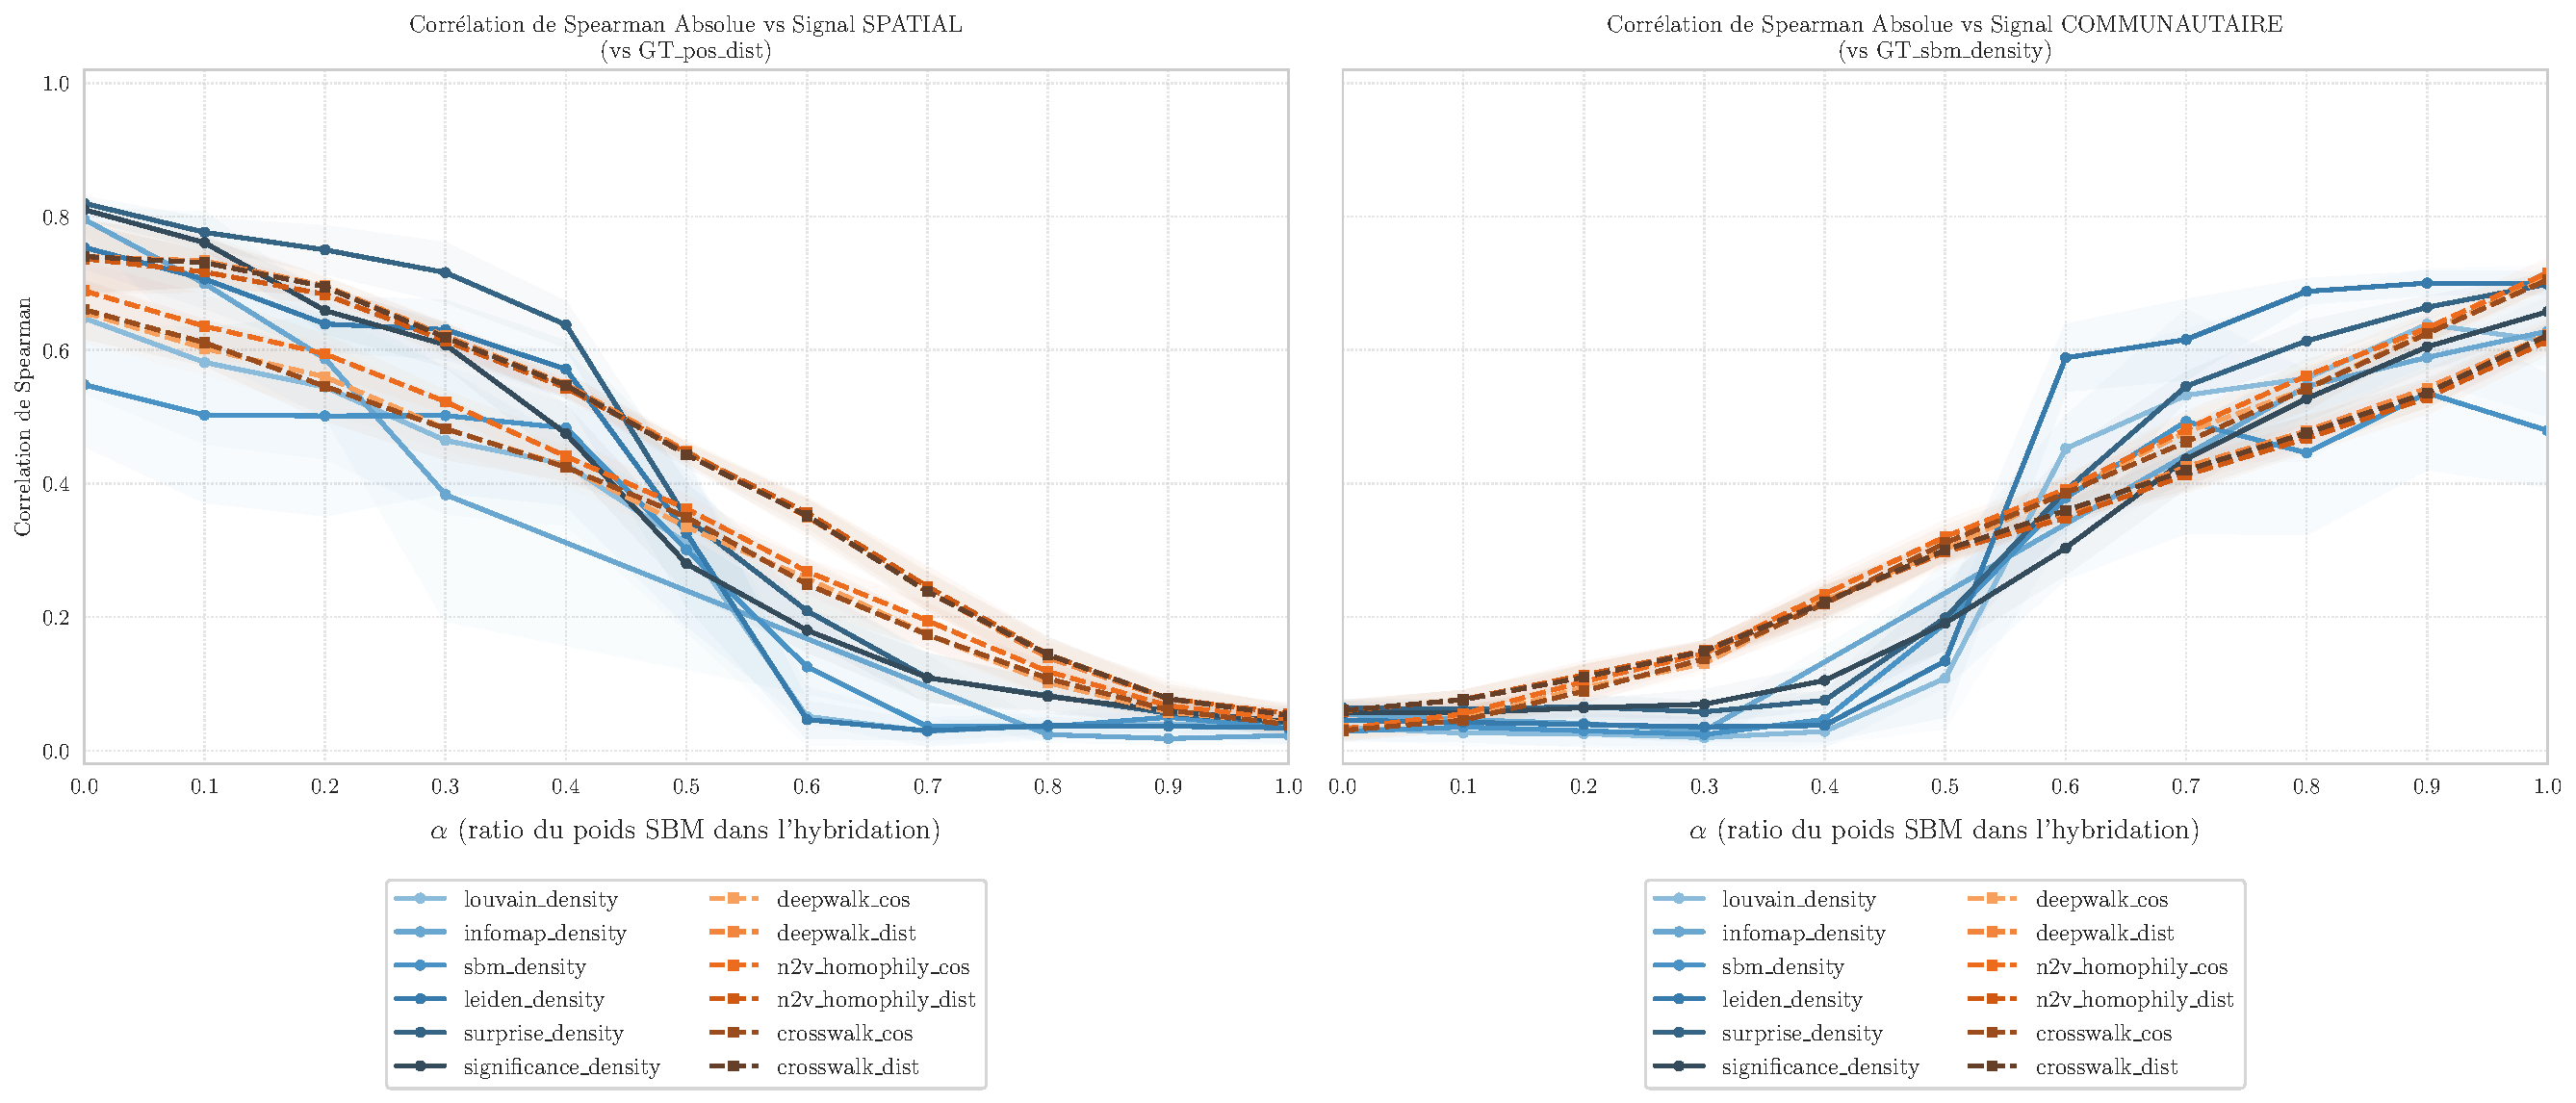
\includegraphics[width=\textwidth]{Plots/206 00_Correl_individual_features_VS_GT_comparison.pdf}
\caption{Evolution du coefficient de spearman entre les features et la \textit{Ground Truth} communautaire (à droite), et la \textit{Ground Truth} géométrique (à gauche) en fonction de $\alpha$ (moyenne sur 10 itérations).} 
\label{fig5}
\end{figure}


\subsection{Redondance entre les descripteurs Communautaires et \textit{Embeddings}}

Cette polyvalence géométrico-structurelle traduit également le fait que ces deux familles de descripteurs souffrent d'une forte redondance informationnelle. Afin de quantifier précisément ce chevauchement, le Tableau~\ref{tab:collinearity_alpha} synthétise l'évolution de la corrélation de Spearman moyenne calculée sur l'ensemble des paires de caractéristiques issues des paradigmes communautaire et géométrique ($6 \times 6$ paires car 6 variables pour chaque paradigme).

\begin{table}[!ht]
\centering
\caption{Évolution de la colinéarité moyenne inter-paradigme (Spearman) en fonction de $\alpha$ avec un intervalle de confiance à 95\,\% (10 itérations)}
\label{tab:collinearity_alpha}
\begin{tabular}{cc}
\hline
\textbf{Ratio SBM ($\alpha$)} & \textbf{Corrélation Moyenne Inter-Groupe $|\rho| \pm \text{IC}_{95\%}$} \\
\hline
1,0 & 0,6166 $\pm$ 0,0210 \\
0,9 & 0,5392 $\pm$ 0,0205 \\
0,8 & 0,4409 $\pm$ 0,0143 \\
0,7 & 0,3993 $\pm$ 0,0068 \\
0,6 & 0,3403 $\pm$ 0,0111 \\
0,5 & 0,3133 $\pm$ 0,0072 \\
0,4 & 0,3978 $\pm$ 0,0125 \\
0,3 & 0,4535 $\pm$ 0,0250 \\
0,2 & 0,5157 $\pm$ 0,0182 \\
0,1 & 0,5768 $\pm$ 0,0134 \\
0,0 & 0,6330 $\pm$ 0,0184 \\
\hline
\end{tabular}
\end{table}

Son analyse montre que la colinéarité inter-groupe décrit une courbe convexe symétrique, atteignant un minimum à $\alpha = 0,5$ avec une corrélation absolue moyenne de $0,3133 \pm 0,0072$. À mesure que le réseau se polarise vers l'un des deux générateurs purs, cette corrélation s'exacerbe et devient hautement significative, culminant à $0,6166 \pm 0,0210$ pour le pôle communautaire ($\alpha = 1,0$) et jusqu'à $0,6330 \pm 0,0184$ pour le pôle spatial ($\alpha = 0,0$). 

Cette colinéarité floute l'explicabilité du modèle en introduisant un effet de confusion : le méta-classificateur ne sépare pas des signaux orthogonaux indicateurs d'un facteur spécifique. Ce verrou méthodologique justifie directement l'introduction, dans le chapitre suivant, de nos approches d'inférence de métriques décorrélées par débiaisage géométrique.



\section{Inférence de représentations structurelles décorrélées}
\label{sec:debiaisage_structurel}

Le constat de redondance informationnelle établi au chapitre précédent met en évidence une limite majeure de l'état de l'art : la difficulté des algorithmes classiques à isoler des facteurs d'influence uniques. Dans l'objectif d'offrir de meilleures perspectives d'explicabilité, ce chapitre introduit deux contributions dédiées à l'inférence de caractéristiques débiaisées, visant à purger les métriques d'une composante déjà identifiée, et en l'occurence de leur composante spatiale.

\subsection{Communautés de Louvain spatialement décorrélées}

La détection de communautés via l'algorithme de Louvain classique \cite{louvain2008}, s'appuie nativement sur le modèle nul de configuration de Newman-Girvan. Ce modèle souffre d'une faiblesse théorique : il suppose que la probabilité de connexion entre deux nœuds ne dépend que de leurs degrés, ignorant toute autre contrainte telle que la distance physique par exemple. En présence d'un réseau hybride géométrico-communautaire, Louvain interprète mécaniquement le regroupement géographique de noeuds interconnectés comme une communauté topologique, créant le biais de confusion observé.

\subsubsection{Inférence du modèle nul gravitaire}
Pour lever ce verrou, l'approche présentée s'inspire directement des travaux de Cazabet et al. \cite{cazabet2022enhancing}, qui injectent un modèle nul spatial contraint par les degrés ($\text{DC-Spatial}$) directement au cœur du critère d'optimisation de l'algorithme de Louvain. La spécificité de la méthode proposée est que le Null Modèle spatial utilisé est directement inféré à partir du graphe étudié lui même.
Pour cela, nous inférons un modèle gravitaire dont la probabilité d'existence d'un lien est gouvernée par des potentiels de nœuds $\alpha$ (degrés latents) et un paramètre d'échelle global $\beta$ pondérant l'impact de la distance sur la connexion des noeuds. La matrice de probabilité du modèle nul $P$ est inférée par maximum de vraisemblance via un algorithme itératif de descente de coordonnées, combiné à une méthode de Newton :

\begin{equation}
    P_{uv} = \frac{1}{1 + e^{-(\alpha_u + \alpha_v - \beta \cdot d_{uv})}}
\end{equation}

Les paramètres nodaux $\alpha$ ajustent la contrainte sur les degrés attendus, tandis que l'optimisation scalaire de $\beta$ maximise la log-vraisemblance globale sur le triangle supérieur de la matrice d'adjacence $A$. Pour garantir la symétrie stricte exigée par le calcul de modularité, la matrice finale du modèle nul est définie par $P^{\text{sym}} = (P + P^T)/2$.

\subsubsection{Optimisation de la modularité ignorant l'influence spatiale}

Cette matrice $P^{\text{sym}}$ est ensuite substituée au modèle nul classique au sein de l'algorithme \texttt{MetaLouvain}, développé dans les travaux de Rémy Cazabet. La nouvelle fonction de modularité modifiée évalue l'écart entre la topologie observée et les prédictions du modèle nul gravitaire où $A_{uv}$ désigne un élément de la matrice d'adjacence du réseau, et $b_u$ et $b_v$ les identifiants des communautés respectives des nœuds $u$ et $v$~:

\begin{equation}
\label{eq:q_spatial}
    Q_{\text{Spatial}} = \frac{1}{2m} \sum_{u,v} \left( A_{uv} - P^{\text{sym}}_{uv} \right) \mathbb{I}(b_u = b_v)
\end{equation}

En soustrayant la probabilité de liaison capturée par le modèle nul géométrique, le modèle ne considère comme significatives que les arêtes qui s'établissent au-delà des attentes gravitaires. Les communautés ainsi extraites découlent d'un signal d'affinité topologique pure (et de résidus statistiques, ou bruit), purgé de l'effet de proximité géographique dans la mesure de ce que le modèle nul parvient à capturer.


\subsection{Plongements géométriques type SiNE spatialement décorrélés}

Si l'approche précédente montre des résultats intéressants (voir partie \ref{sec:5_3Validafion}), elle se heurte à une faiblesse intrinsèque des algorithmes de partitionnement : le besoin d'un fort signal de densité pour converger vers des blocs stables. Pour capturer des signaux d'affinité plus diffus, nous basculons vers une nouvelle approche en transposant le concept de décorrélation au sein des plongements de graphes (\textit{graph embeddings}).

\subsubsection{Formulation de la matrice de résidus}
Plutôt que d'apprendre des représentations sur la matrice d'adjacence brute $A$, notre méthode, baptisée $\text{SiNE décorrelée}$, opère sur la \textbf{matrice de résidus} structurels $R$, définie par la soustraction du modèle nul gravitaire inféré précédemment :
\begin{equation}
    R = A - P^{\text{sym}}
\end{equation}
Cette opération transforme le réseau en un graphe signé virtuel où $R_{uv} \ge 0$ traduit une sur-représentation topologique (affinité positive) et $R_{uv} < 0$ une sous-représentation (répulsion négative) par rapport à la contrainte spatiale.

\subsubsection{Échantillonnage stochastique par Softmax}
Pour guider l'apprentissage, nous implémentons un protocole d'échantillonnage de paires dyadiques basé sur l'intensité des résidus. Pour chaque nœud $i$, les candidats valides font l'objet d'un tirage aléatoire sans remise pondéré par une distribution Softmax appliquée sur la valeur absolue des résidus $|R_{ij}|$, modulée par un paramètre de température $T$ :
\begin{equation}
    p(j \mid i) = \frac{e^{|R_{ij}| / T}}{\sum_{w \in \mathcal{V}_i} e^{|R_{iw}| / T}}
\end{equation}
Ce mécanisme force l'algorithme à focaliser son attention sur les dyades qui manifestent les plus fortes déviations (positives ou négatives) vis-à-vis du modèle nul.

\subsubsection{Optimisation par perte de signe paire-à-paire} La complexité de la méthode réside dans le fait d'avoir à gérer des pondérations de liens positives comme négatives. Pour résoudre ce problème, les plongements continus en dimension $d=64$ sont optimisés de bout en bout via une fonction de perte antagoniste signée (\textit{Pairwise Sign Loss}) entraînée par l'optimisateur Adam (mécanisme inspiré des travaux de Daokun Zhang et al. \cite{wang2017SINE}). Soit $\mathbf{z}_u$ le vecteur latent du nœud $u$, la fonction de coût minimise la distance euclidienne pour les résidus positifs et applique une marge de séparation stricte ($m=2,0$) pour les résidus négatifs :
\begin{equation}
    \mathcal{L} = \mathbb{E}_{(u,v) \sim \mathcal{S}} \left[ \mathbb{I}(R_{uv} \ge 0) \|\mathbf{z}_u - \mathbf{z}_v\|_2 + \mathbb{I}(R_{uv} < 0) \max\left(0, m - \|\mathbf{z}_u - \mathbf{z}_v\|_2\right) \right]
\end{equation}

\subsection{Validation des résultats et analyse et performances empiriques}
\label{sec:5_3Validafion}

\subsubsection{Validation du fonctionnement des algorithmes}

La validation des méthodes proposées repose, dans un premier temps, sur l'évaluation de l'indépendance statistique entre les partitions et représentations latentes obtenues, vis-à-vis de la vérité terrain $\text{GT\_pos}$ par rapport à laquelle elles ont été décorrélées.

\begin{figure}
\includegraphics[width=\textwidth]{Plots/207 02_Correl_All_SBM_and_POS.png}
\caption{Evolution du coefficient de spearman entre chaque feature standard et débiaisée, et la \textit{Ground Truth} communautaire (à droite), ou la \textit{Ground Truth} géométrique (à gauche) en fonction de $\alpha$ (moyenne sur 10 itérations).} 
\label{fig6}
\end{figure}

\begin{figure}
\includegraphics[width=\textwidth]{Plots/208 02_MI_adjusted_All.png}
\caption{Evolution de l'Information Mutuelle Ajustée (AMI) entre chauque features standard et débiaisée, et la \textit{Ground Truth} communautaire (à droite), ou la \textit{Ground Truth} géométrique (à gauche) en fonction de $\alpha$ (moyenne sur 10 itérations).} 
\label{fig8}
\end{figure}

L'analyse des corrélations de Spearman (Figure \ref{fig6}) et de l'Information Mutuelle Ajustée (Figure \ref{fig8}) confirme que l'algorithme de Louvain décorrélé remplit pleinement ses objectifs théoriques. En effet, nous observons une corrélation quasi-nulle avec la vérité terrain spatiale ($\text{GT\_pos}$) sur la quasi-totalité des ratios d'hybridation $\alpha$. Une légère augmentation de cette corrélation est perceptible uniquement autour du point extrême $\alpha = 0$, configuration où l'information spatiale constitue l'unique source de structure du réseau. De plus, la corrélation et l'information mutuelle capturées avec la structure communautaire cible ($\text{GT\_sbm}$) sont améliorées sur la plage intermédiaire $0.2 \le \alpha \le 0.5$.

Des tendances similaires sont observées pour les plongements (\textit{embeddings}) issus de $\text{SiNE}$ décorrélé. Ces derniers présentent une corrélation et une quantité d'information mutuelle plus faibles avec la composante spatiale $\text{GT\_pos}$ que les plongements de référence générés par la méthode classique DeepWalk, et ce pour l'ensemble des valeurs de $\alpha$. Par ailleurs, le mécanisme de décorrélation permet à la méthode proposée de s'aligner plus fidèlement sur la structure $\text{GT\_sbm}$ de par une plus haute corrélation, sans pour autant capturer plus d'information mutuelle.

Ces premières observations valident empiriquement le comportement de nos deux approches : elles permettent d'inférer des structures communautaires (pour Louvain décorrélé) et des représentations vectorielles (pour SiNE décorrélé) significativement plus orthogonales à la topologie spatiale que les méthodes standards de la littérature.

\subsubsection{Performance des algorithmes par rapport à l'état de l'art}

Dans un second temps, afin d'évaluer la pertinence et l'apport applicatif de ces approches débiaisées, nous mesurons leurs performances dans une tâche de prédiction de liens. L'objectif est de comparer l'efficacité de l'association des descripteurs décorrélés avec la \textit{Ground Truth} spatiale ($\text{GT\_pos}$ + métrique décorrélée) face à celles des standards de l'état de l'art ($\text{GT\_pos}$ + Louvain classique, ou $\text{GT\_pos}$ + DeepWalk). Cette évaluation permet de vérifier si l'extraction d'une information plus orthogonale offre une meilleure complémentarité, et donc une meilleure compréhension de la topologie globale du graphe.

Sur les graphes générés par une hybridation par somme pondérée, les performances entre le modèle de base ($\text{GT\_pos} + \text{Louvain standard}$) et notre variante débiaisée ($\text{GT\_pos} + \text{Louvain décorrélé}$) s'avèrent très proches (Figure \ref{fig:10.1}). Néanmoins, une amélioration statistiquement significative (évaluée sur 30 itérations avec un intervalle de confiance à $95\,\%$) émerge précisément au point critique $\alpha = 0.5$. Cette zone correspond au point de transition où le conflit d'information entre géométrie et communautés est maximal, démontrant l'intérêt de la décorrélation lorsque les signaux sont très entremêlés. Sur le reste du spectre de $\alpha$, la méthode débiaisée fait jeu égal avec la référence.

Cette dynamique se confirme, de manière plus marquée, sur les graphes hybridés par la méthode dite "exposant" (Figure \ref{fig:10.2}). Cette hybridation génère des structures plus contrastées où l'apport de chaque composante est plus net. Dans cette configuration, l'approche décorrélée surclasse de manière significative l'état de l'art sur une large plage de ratios, pour $0.3 \le \alpha \le 0.7$.

Les performances sur les mêmes setups de SiNEcustom en prédiction de liens, donnent des résultats encore plus encourageants : SiNE custom + GT\_pos bat deepwalk + GT\_pos pour les aplhas entre 0.5 et 1.0, avec le plus gros écart sur 0.7, sur les hybrides par somme (Figure \ref{fig:10.3}). ET sur les hybrides par méthode exposant, ils font mieux dès 0.2 jusqu'à 1.0. On pourrait aussi dire 2-3 trucs sur la forme des courbes, mais un peu osef pour notre problématique.


Enfin, les évaluations menées sur l'algorithme $\text{SiNE}$ décorrélé révèlent des résultats encore plus prometteurs. Pour les graphes hybridés par somme (Figure \ref{fig:10.3}), la combinaison $\text{SiNE décorrélé} + \text{GT\_pos}$ surclasse le couple $\text{DeepWalk} + \text{GT\_pos}$ sur l'intervalle $0.5 \le \alpha \le 1.0$, l'écart de performance maximal étant atteint pour $\alpha = 0.7$. Enfin, sur les variantes de graphes par exposant (Figure \ref{fig:10.4}), la méthode proposée surpasse la référence sur la quasi-totalité des hybrides, dès le seuil de $\alpha = 0.2$ et jusqu'à $\alpha = 1.0$.


\begin{figure}[htbp]
    \centering
    % --- Première ligne (Plots côte à côte) ---
    \begin{minipage}[b]{0.48\textwidth}
        \centering
        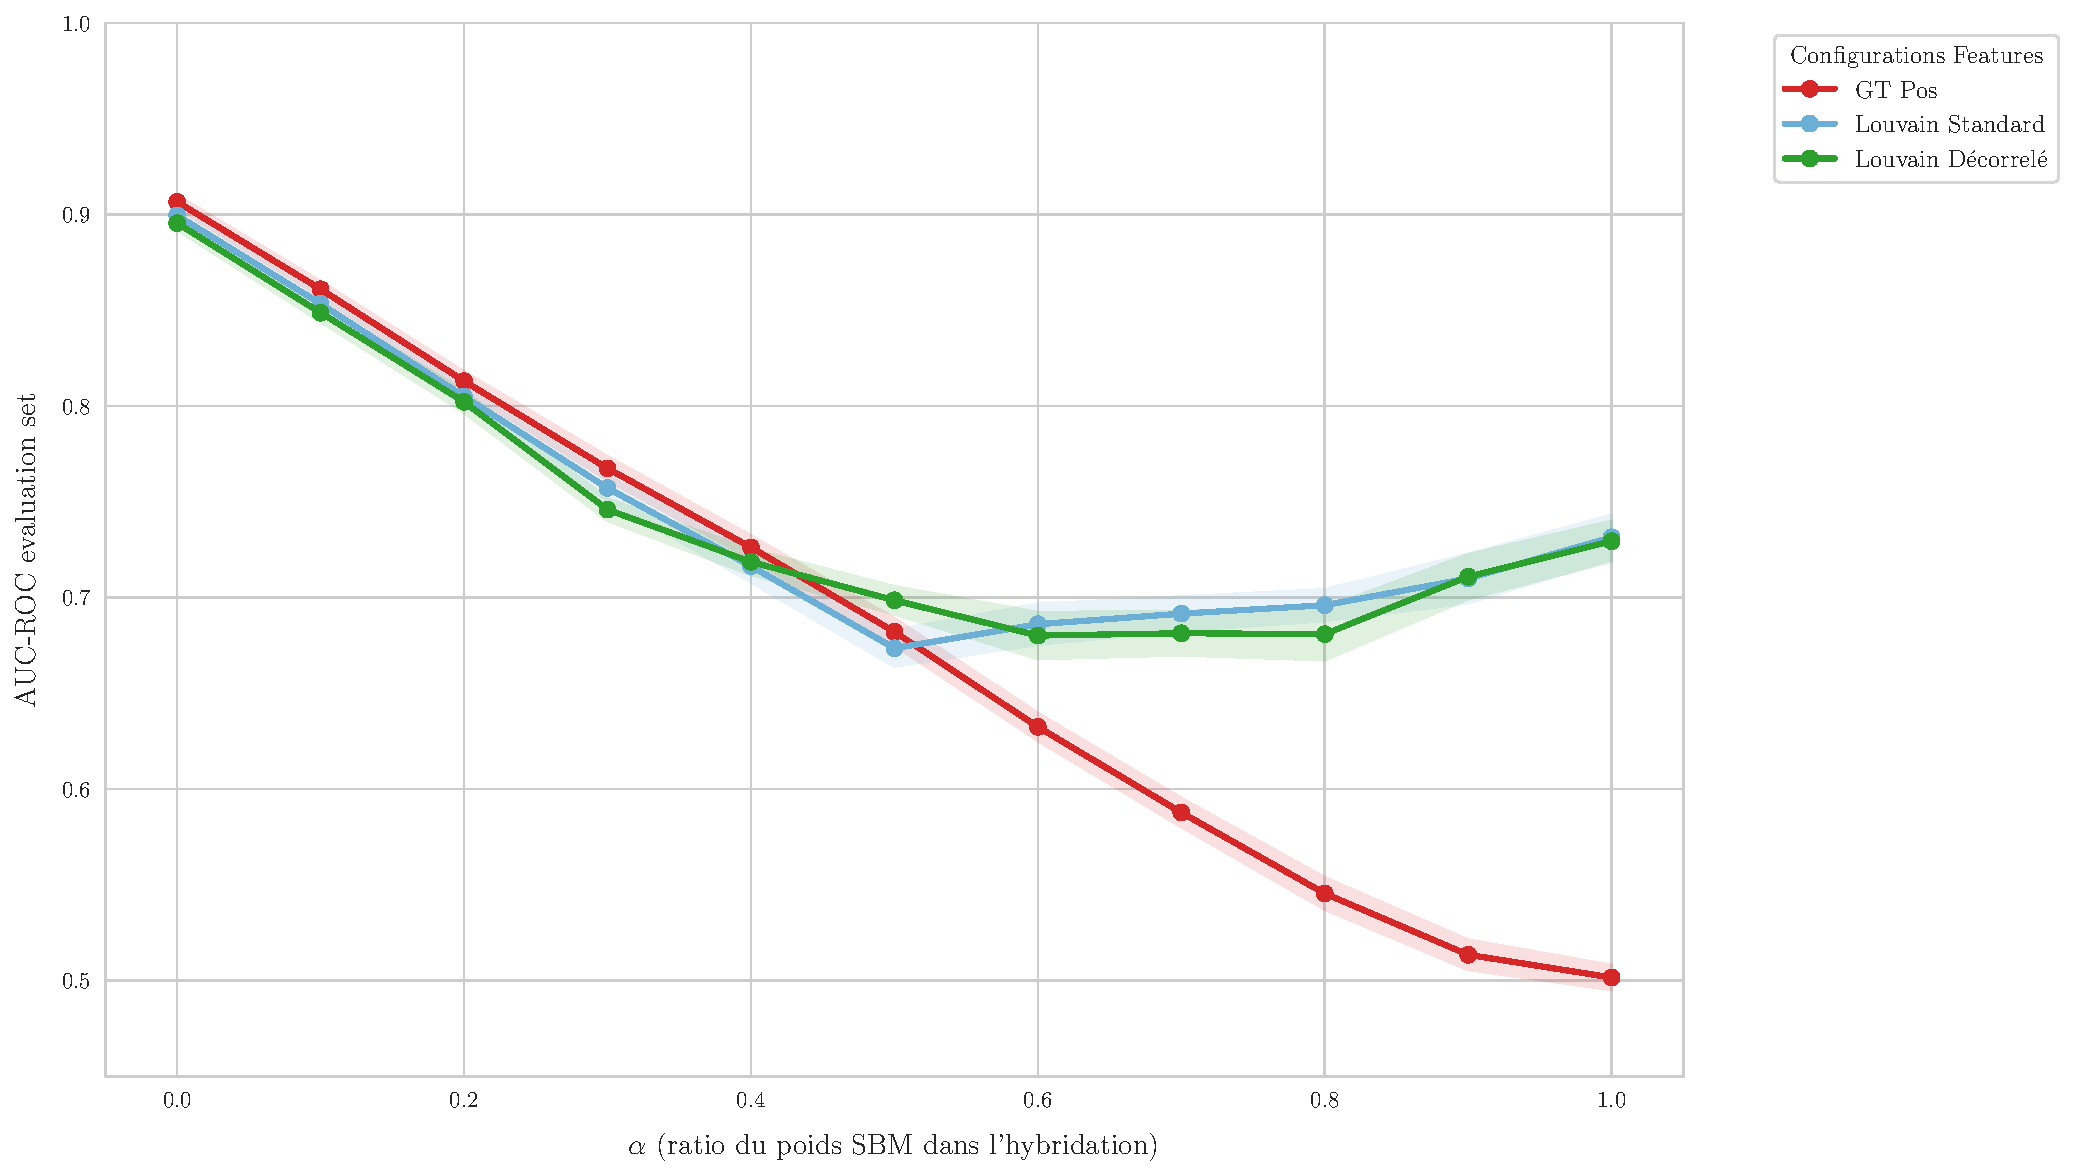
\includegraphics[width=\textwidth]{Plots/209 01_artificial_graphs_shuffled_v4_comuAndEmb_30iter_GTposAndComu_20260529_AUC-ROC_eval_CI99_SBM_ratio.pdf}
        \caption{(a) Louvain Standard vs Décorrelé (hybridation par somme pondérée)}
        \label{fig:10.1}
    \end{minipage}
    \hfill
    \begin{minipage}[b]{0.48\textwidth}
        \centering
        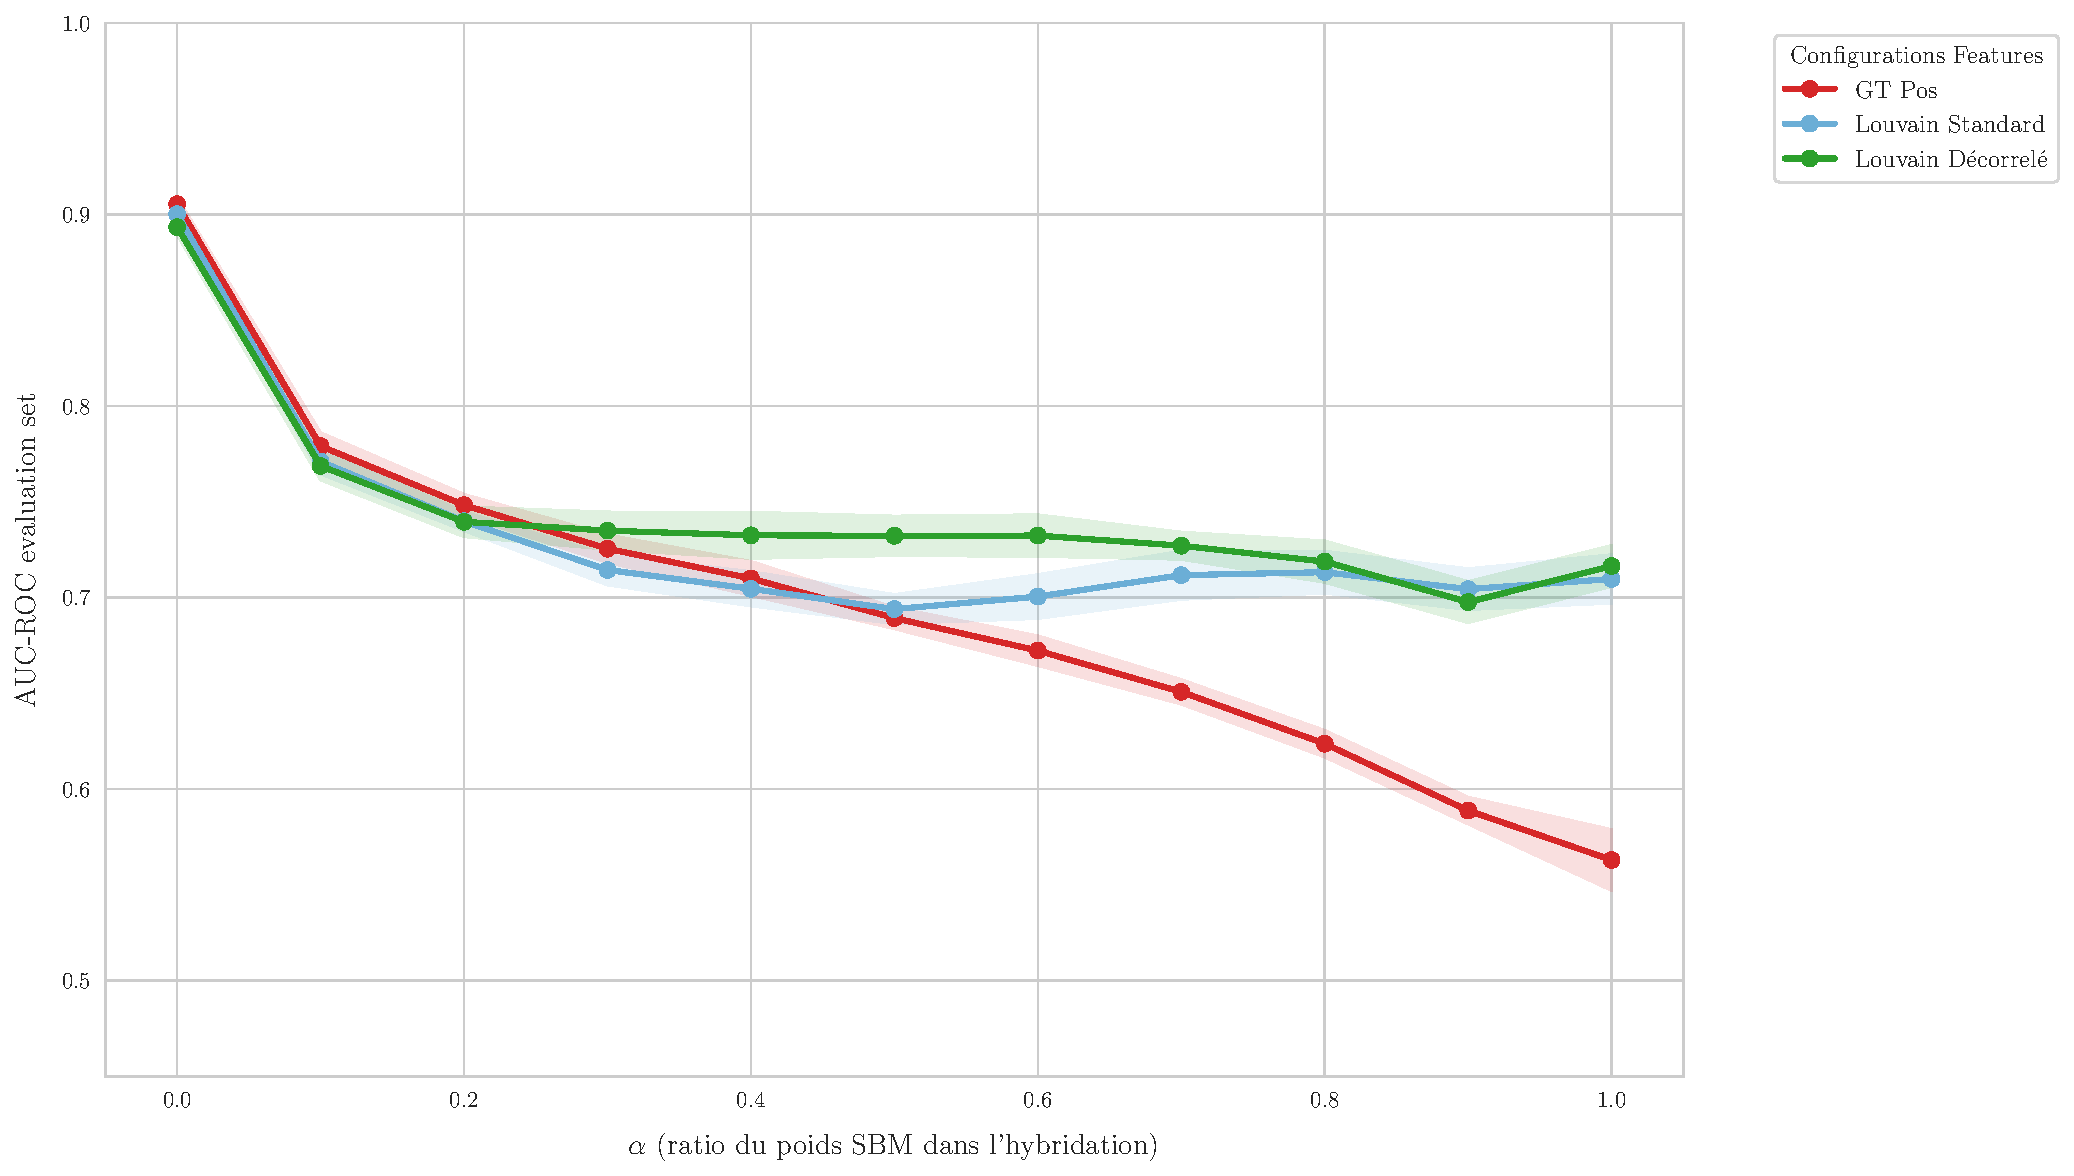
\includegraphics[width=\textwidth]{Plots/211 01_artificial_graphs_shuffled_v6_comuAndEmb_30iter_GTposAndComu_20260529_AUC-ROC_eval_CI99_SBM_ratio.pdf}
        \caption{(b) Louvain Standard vs Décorrelé (hybridation exponentielle)}
        \label{fig:10.2}
    \end{minipage}

    \vspace{0.5cm} % Espace vertical entre les deux lignes

    % --- Deuxième ligne (Plots côte à côte) ---
    \begin{minipage}[b]{0.48\textwidth}
        \centering
        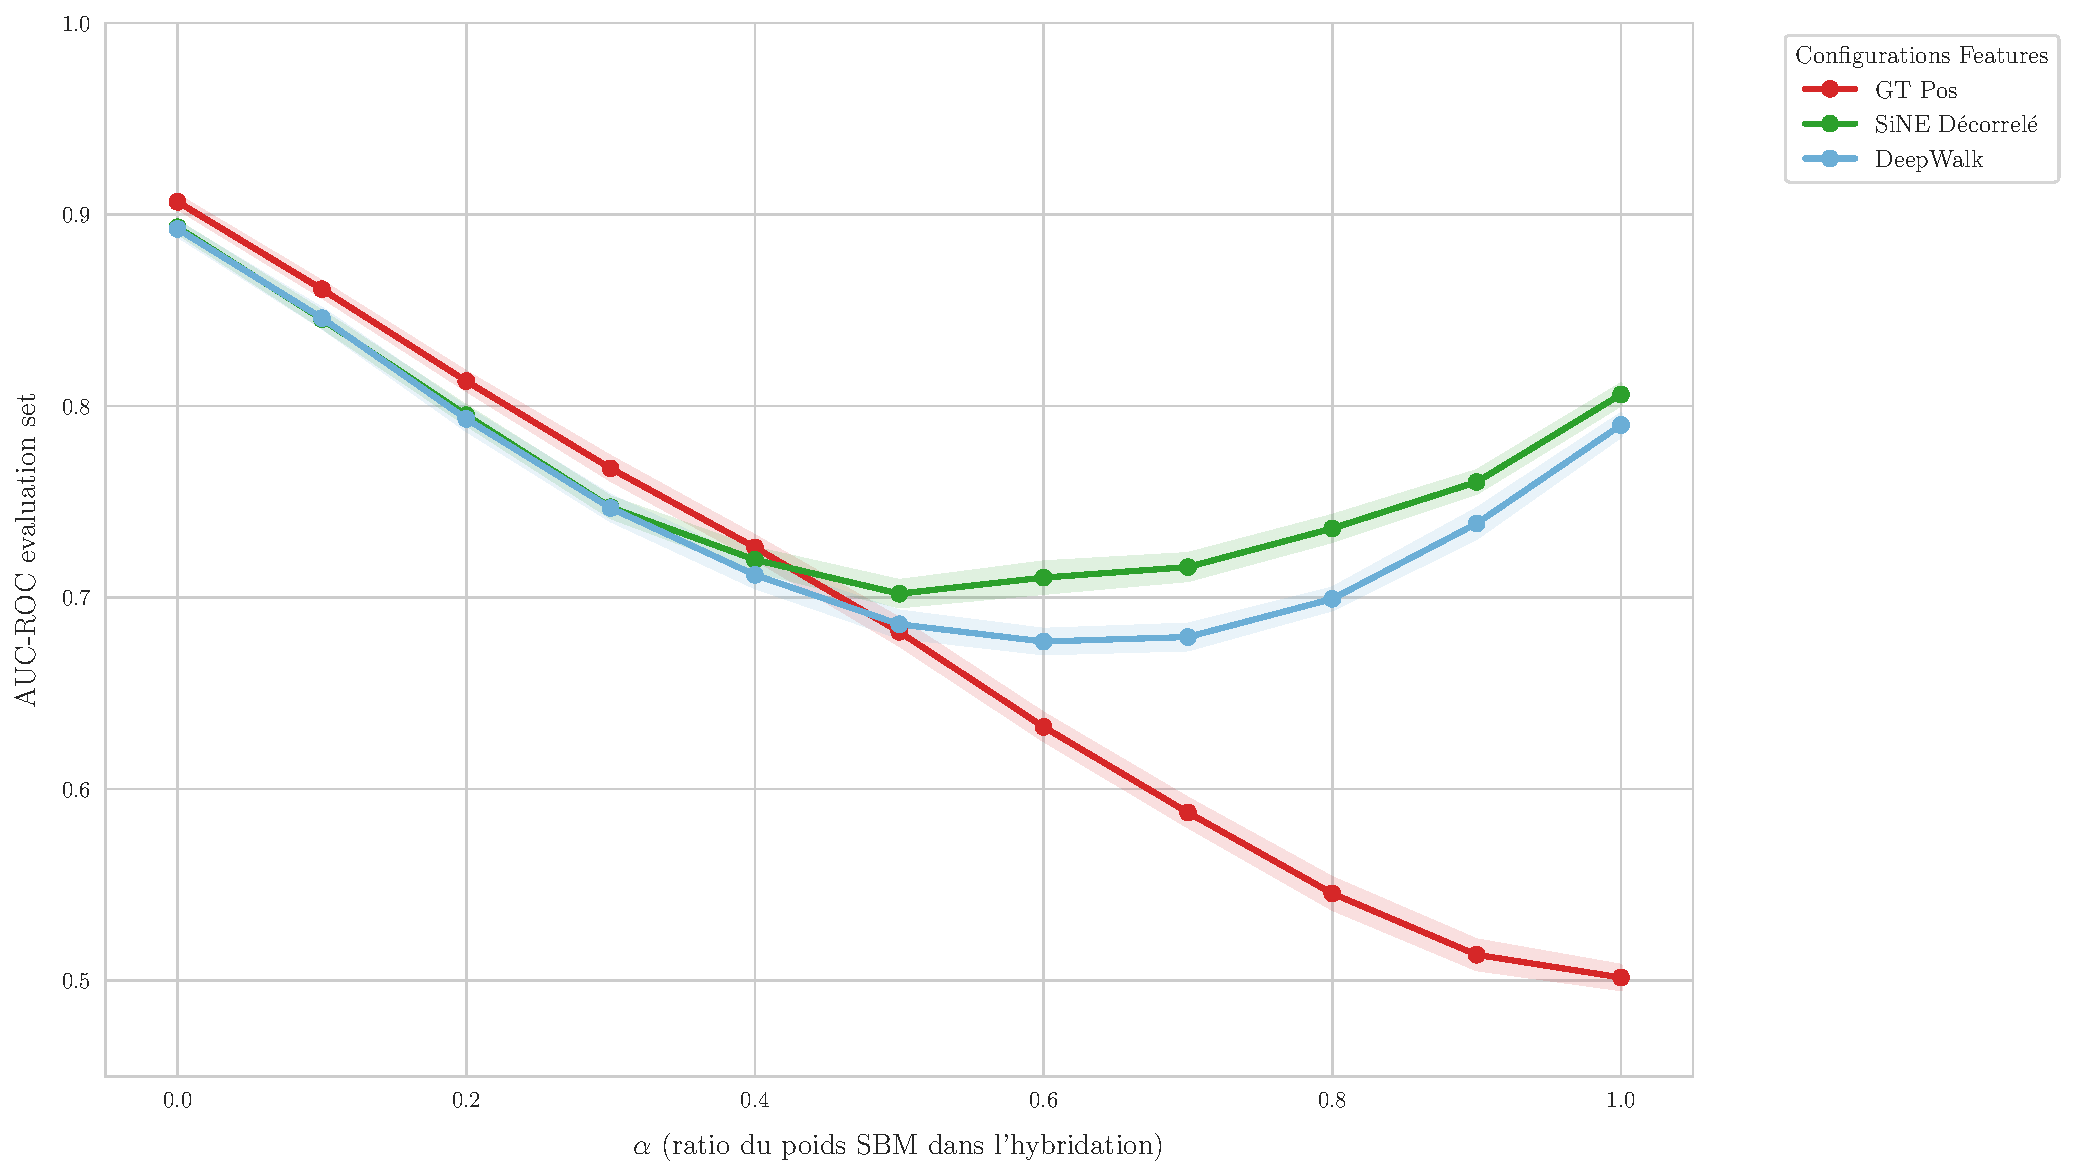
\includegraphics[width=\textwidth]{Plots/210 01_artificial_graphs_shuffled_v4_comuAndEmb_30iter_GTposAndSine_20260529_AUC-ROC_eval_CI99_SBM_ratio.pdf}
        \caption{(c) DeepWalk vs SiNE Décorrélée (hyb. par somme pondérée)}
        \label{fig:10.3}
    \end{minipage}
    \hfill
    \begin{minipage}[b]{0.48\textwidth}
        \centering
        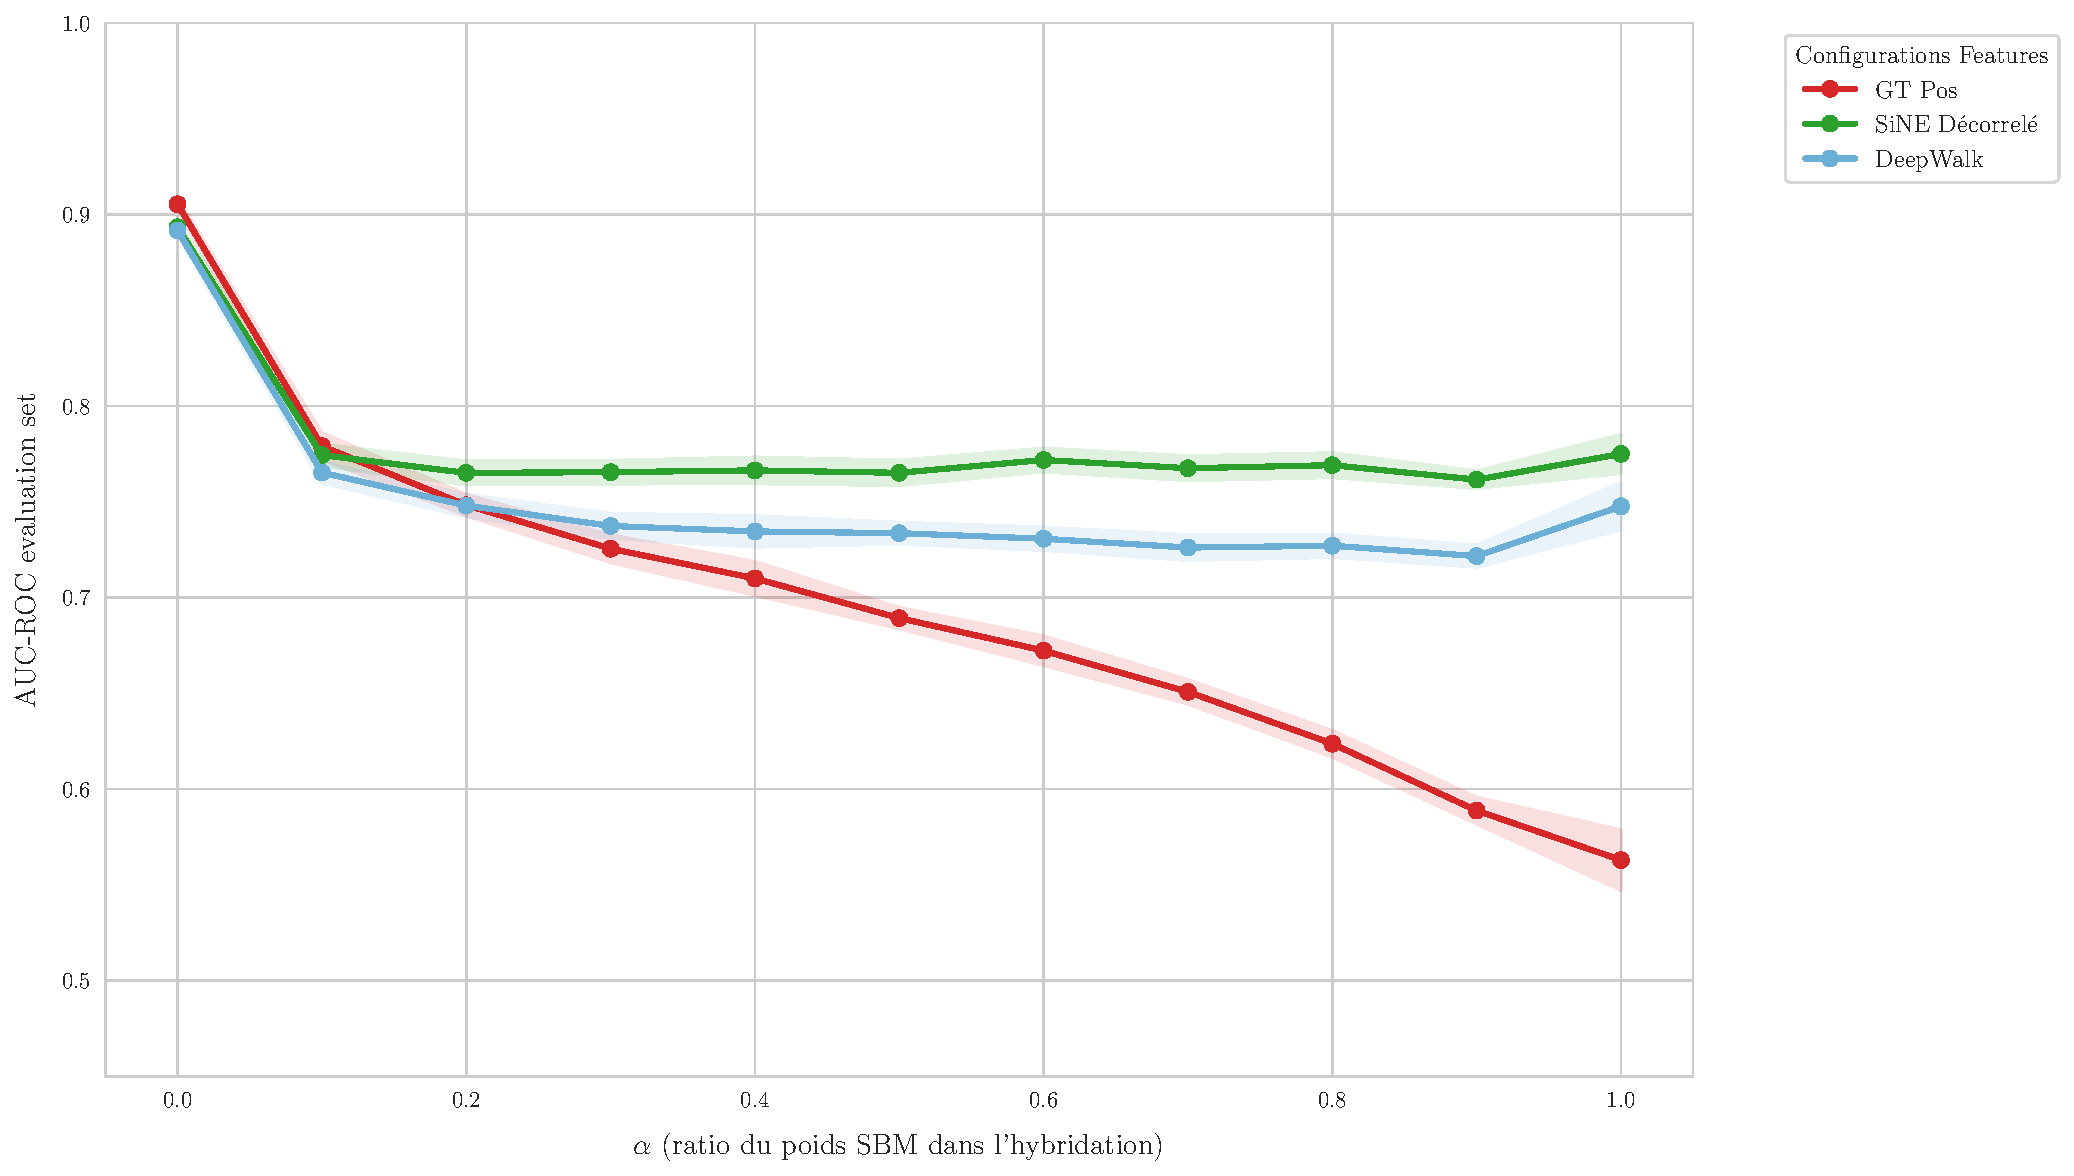
\includegraphics[width=\textwidth]{Plots/212 01_artificial_graphs_shuffled_v6_comuAndEmb_30iter_GTposAndSine_20260529_AUC-ROC_eval_CI99_SBM_ratio.pdf}
        \caption{(d) DeepWalk vs SiNE Décorrélée (hybridation exponentielle)}
        \label{fig:10.4}
    \end{minipage}

    % Légende générale requise par Springer
    \caption{Evolution de l'AUC-ROC du modèle de prédiction de lien \protect\textit{XGBoost} entraîné à l'aide de le \textit{Ground Truth} spatiale et des features standard ou débiaisées (sur 30 itérations).}
    \label{fig:fig10}
\end{figure}




\section{Discussion, Conclusions et Perspectives Générales}
\label{sec:discussion_conclusion}

Cette section synthétise les contributions développées au cours de ce projet de recherche, analyse de manière critique sa portée et ses limites actuelles, et propose des axes de développement futurs.

\subsection{Discussion synthétique des contributions}

Le fil conducteur du projet reposait sur l'utilisation de la prédiction de liens comme outil d'analyse pour évaluer la qualité et l'indépendance de représentations de graphes. Les apports de ces travaux s'articulent autour de trois axes majeurs :

\begin{enumerate}
    \item \textbf{La maîtrise du benchmark de validation :} Avant d'analyser l'état de l'art, le développement d'un modèle génératif hybride (SBM-Spatial) a mis en lumière un verrou mathématique critique. Nous avons démontré théoriquement et numériquement que le simple mélange linéaire de deux matrices de probabilités biaise l'échantillonnage en faveur du modèle possédant la plus forte variance. L'alignement algorithmique des variances via l'optimisation du paramètre de dissuasion $\sigma^*$ a permis de concevoir un cadre de validation rigoureux, symétrique et exempt de biais de filiation.
    \item \textbf{La mise en évidence du biais de colinéarité :} L'application du framework d'explicabilité additive inspiré de SHAP a validé notre démarche sur des variables parfaites ($\text{GT\_pos}$ et $\text{GT\_sbm}$). Cependant, face aux algorithmes de l'état de l'art, le framework a révélé une forte redondance informationnelle inter-paradigme (culminant à plus de $60\,\%$ de corrélation aux bornes du spectre). Ce phénomène de colinéarité induit un effet de masquage lors de l'apprentissage par arbres (\textit{XGBoost}), concentrant artificiellement l'importance SHAP vers un nombre restreint de descripteurs et floutant l'interprétabilité globale. De plus, le comportement des algorithmes classiques a confirmé un biais conceptuel : Louvain interprète la proximité géographique locale comme une structure communautaire, et inversement les algorithmes d'inférence de positions latentes type \textit{embeddings} détectent les structures communautaires comme de la proximité géographique.
    \item \textbf{L'efficacité du débiaisage par modèle nul :} Pour répondre à cette limite, les méthodes d'inférence décorrélée développées (Louvain spatialement décorrélé et SiNE décorrélée via matrice de résidus) ont prouvé leur capacité à purger efficacement le signal de sa composante géométrique. L'effondrement des corrélations avec $\text{GT\_pos}$ (Figures \ref{fig6} et \ref{fig8}) valide l'orthogonalisation des descripteurs. En termes de performance applicative, cette séparation des signaux s'est avérée particulièrement intéressante dans les zones de forte incertitude ($\alpha = 0.5$ pour le modèle par somme) et sur l'ensemble du spectre pour les structures contrastées (modèle par exposant), confirmant qu'isoler des facteurs d'influence uniques permet au méta-classificateur de mieux reconstruire la topologie globale.
\end{enumerate}

\subsection{Limites actuelles et verrous technologiques}

Malgré des résultats encourageants, plusieurs limites doivent être soulignées. En premier lieu, la validation des performances s'est concentrée sur des structures non corrigées des degrés ($\text{non-DC}$). Bien que les formulations mathématiques intégrant l'hétérogénéité des degrés ($\text{DC-SBM}$ et $\text{DC-Spatial}$) aient été implémentées et formalisées dans ce rapport, leur évaluation au sein du framework d'explicabilité reste incomplète, constituant une zone d'ombre sur la robustesse des dynamiques observées sur une \textit{Ground Truth} combinant distance et degré des noeuds.

Deuxièmement, l'évaluation s'est focalisée sur des réseaux synthétiques contrôlés. Si ce choix était indispensable pour valider la fidélité de la décomposition face à une vérité terrain connue, la robustesse de la décorrélation face au bruit, à l'incomplétude ou aux topologies complexes propres aux graphes réels reste encore à valider.

\subsection{Perspectives de recherche et développements futurs}

Les pistes explorées au cours de ce projet ouvrent de nouveaux questionnements. Voici les principales perspectives et pistes de recherche qu'il paraît intéressant de poursuivre : 

\subsubsection{Passage à l'échelle et validation sur graphes réels}
C'est la suite logique de ce travail, qui réside dans la conduite d'une expérimentation sur des jeux de données réels à grande échelle. Les analyses isolées menées en fin de projet devront être généralisées à des réseaux complexes issus de domaines variés, tels que les réseaux de transport (où la contrainte spatiale est forte), les réseaux de citations ou les réseaux sociaux géolocalisés. Il s'agira de vérifier si les modèles nuls gravitaires maintiennent leur capacité de décorrélation face à des structures empiriques sur lesquelles les facteurs influençant la création de liens sont multiples (plus que 2 paradigmes).

\subsubsection{Optimisation algorithmique et ingénierie logicielle}
D'un point de vue informatique, notre implémentation personnalisée de l'algorithme SiNE ($\text{SiNEcustom}$), codée en Python pour les besoins de cette preuve de concept, présente des limites de montée en charge. Le calcul des fonctions de perte avec contraintes d'orthogonalité sur des matrices de résidus signés s'avère gourmand en ressources. 
Une réécriture des modules critiques en C++, ou une intégration au sein de frameworks de calcul parallélisé sur GPU (tels que PyTorch ou JAX), s'avère indispensable pour réduire les temps de calcul, optimiser la convergence du gradient et garantir la scalabilité du modèle sur des graphes de plusieurs millions de nœuds.

\subsubsection{Généralisation théorique et Équité (\textit{Fairness})}
Enfin, sur le plan théorique, le principe de décorrélation par soustraction de modèle nul formalisé dans ce stage ne se limite pas à la variable géographique. Une perspective majeure consiste à transposer cette méthodologie pour débiaiser les plongements ou les partitions vis-à-vis d'autres propriétés structurelles (comme le degré des nœuds pour éviter la sur-représentation des \textit{hubs}) ou vis-à-vis d'attributs temporels, ou encore d'attributs externes sensibles. Ce cadre algorithmique offre par exemple des connexions prometteuses avec le domaine de l'équité en apprentissage sur graphes (\textit{Fair Graph Learning}), où l'objectif est d'extraire des représentations vectorielles rigoureusement orthogonales à des variables protégées (genre, ethnie, données privées) afin de garantir des prédictions non biaisées. De même, l'injection d'un modèle nul communautaire de type \textit{Stochastic Block Model} (\text{SBM}), ouvrirait la voie à une extraction des résidus géométriques, rigoureusement affranchie des effets de regroupement en blocs.


\subsection{Conclusion du stage}

Ce stage de fin d'études, mené au sein de l'équipe DM2L du LIRIS, a permis de poser les bases d'une approche d'explicabilité structurelle et globale pour l'analyse de réseaux. En s'éloignant des explications locales traditionnelles par sous-graphes, ces travaux démontrent qu'il est possible de quantifier finement les facteurs d'influence d'un graphe en combinant la puissance prédictive de la méthode \textit{XGBoost} et la théorie des jeux coopératifs. 

L'introduction de méthodes d'inférence décorrélées résout un verrou critique de colinéarité, ouvrant la voie à des modèles d'apprentissage de représentations sur graphes plus transparents, plus robustes et plus interprétables.
    
\begin{credits}
\subsubsection{Remerciements:} merci à Rémy Cazabet, encadrant de ce stage, pour ses conseils et sa guidance tout au long du projet. Merci à lui de s'être rendu disponible pour de longs échanges hebdomadaires toujours passionants, même depuis l'autre bout du monde, qui n'ont pû que confirmer mon goût pour la recherche. Travailler avec lui sur ce projet a été un véritable plaisir et ces 5 mois sont passés en un clin d'oeil. Merci aux collègues doctorants, post-doctorants et stagiaires du LIRIS d'avoir égayé mes journées, ainsi qu'aux permanents avec qui j'ai pu échanger. Enfin, merci au laboratoire, à ses responsables et volontaires, de mettre à disposition ce cadre et les moyens de mener à bien nos recherches.
\end{credits}

% ---- Bibliography ----
\begin{thebibliography}{8}

\bibitem{lordShapleyOriginal_1953}
Shapley, L. S.: A Value for n-Person Games. Contributions to the Theory of Games \textbf{2}, 307--318 (1953)

\bibitem{SHAPimplementation_2010}
Štrumbelj, E., Kononenko, I.: An Efficient Explanation of Individual Model Predictions Using Shapley Value Explanations. Machine Learning \textbf{81}(1), 1--18 (2010)

\bibitem{01stackingLinkPred}
Ghasemian, A., Hosseinmardi, H., Galstyan, A., Clauset, A.: Stacking Models for Nearly Optimal Link Prediction in Complex Networks. Proceedings of the National Academy of Sciences \textbf{117}(37), 22777--22785 (2020)

\bibitem{louvain2008}
Blondel, V. D., Guillaume, J. L., Lambiotte, R., Lefebvre, E.: Fast unfolding of communities in large networks. Journal of Statistical Mechanics: Theory and Experiment \textbf{2008}(10), P10008 (2008)

\bibitem{sbm1983}
Holland, P. W., Laskey, K. B., Leinhardt, S.: Stochastic blockmodels: First steps. Social Networks \textbf{5}(2), 109--137 (1983)

\bibitem{deepwalk2014}
Perozzi, B., Al-Rfou, R., Skiena, S.: Deepwalk: Online learning of social representations. In: Proceedings of the 20th ACM SIGKDD International Conference on Knowledge Discovery and Data Mining, pp. 701--710 (2014)

\bibitem{node2vec2016}
Grover, A., Leskovec, J.: node2vec: Scalable feature learning for networks. In: Proceedings of the 22nd ACM SIGKDD International Conference on Knowledge Discovery and Data Mining, pp. 855--864 (2016)

\bibitem{infotheory2023}
Varley, T.F.: Information Theory for Complex Systems Scientists: What, Why, \& How? arXiv preprint arXiv:2304.12482 (2023). 

\bibitem{katz1953}
Katz, L.: A new status index derived from sociometric analysis. Psychometrika \textbf{18}(1), 39--43 (1953)

\bibitem{infomap2008}
Rosvall, M., Bergstrom, C. T.: Maps of random walks on complex networks reveal community structure. Proceedings of the National Academy of Sciences \textbf{105}(4), 1118--1123 (2008)

\bibitem{kipf2016semi}
Kipf, T. N., Welling, M.: Semi-supervised classification with graph convolutional networks. In: Proceedings of the 5th International Conference on Learning Representations (ICLR 2017) (2017)

\bibitem{lichtenwalter2010link}
Lichtenwalter, R. N., Lussier, J. T., Chawla, N. V.: New perspectives and methods in link prediction. In: Proceedings of the 16th ACM SIGKDD International Conference on Knowledge Discovery and Data Mining, pp. 243--252 (2010)

\bibitem{menon2011link}
Menon, A. K., Elkan, C.: Link prediction via matrix factorization. In: Machine Learning and Knowledge Discovery in Databases: European Conference, ECML PKDD 2011, Proceedings, Part II, pp. 437--452 (2011)

\bibitem{taskar2003link}
Taskar, B., Wong, M. F., Abbeel, P., Koller, D.: Link prediction in relational data. In: Advances in Neural Information Processing Systems 16 (NIPS 2003), pp. 659--666 (2003)

\bibitem{ma2024mixture}
Ma, L., Han, H., Li, J., Shomer, H., Liu, H., Gao, X., Tang, J.: Mixture of Link Predictors on Graphs. In: Proceedings of the 30th ACM SIGKDD International Conference on Knowledge Discovery and Data Mining, pp. 2045--2056 (2024)

\bibitem{rahman2019fairwalk}
Rahman, T., Surma, B., Backes, M., Zhang, Y.: Fairwalk: Towards Fair Graph Embedding. In: Proceedings of the 2019 World Wide Web Conference (WWW 2019), pp. 3159--3165 (2019)

\bibitem{khajehnejad2022crosswalk}
Khajehnejad, A., Khajehnejad, M., Babaei, M., Gummadi, K. P., Weller, A., Mirzasoleiman, B.: CrossWalk: Fairness-enhanced Node Representation Learning. In: Proceedings of the AAAI Conference on Artificial Intelligence \textbf{36}(11), 11963--11970 (2022)

\bibitem{schumann2024prejudice}
Schumann, R., et al.: From Prejudice to Parity: A New Approach to Debiasing Large Language Model Word Embeddings. arXiv preprint arXiv:2402.11512 (2024)

\bibitem{zheng2021adversarial}
Zheng, S., Zhu, Z., Liu, Z., Cheng, J., Zhao, Y.: Adversarial Graph Disentanglement with Component-specific Aggregation. IEEE Transactions on Knowledge and Data Engineering \textbf{35}(9), 9234--9247 (2021)

\bibitem{cazabet2022enhancing}
Cazabet, R., Borgnat, P., Jensen, P.: Enhancing Space-Aware Community Detection Using Degree Constrained Spatial Null Model. In: Complex Networks \& Their Applications X, pp. 248--259. Springer (2022)

\bibitem{duvivier2024graph}
Duvivier, L., Cazabet, R., Robardet, C.: Graph space: using both geometric and probabilistic structure to evaluate statistical graph models. In: Proceedings of the 39th ACM/SIGAPP Symposium on Applied Computing (SAC 2024), pp. 1012--1021 (2024)

\bibitem{kamal2025game}
Kamal, A.: Game Theoretic Explainers for Graph Neural Networks. Ph.D. thesis, INSA de Lyon (2025)

\bibitem{fesp2022}
Nisand, G., de Forges, L., Baptiste, P.: Fair and Efficient Alternatives to Shapley-based Attribution Methods. arXiv preprint arXiv:2209.07990 (2022)

\bibitem{karrer2011stochastic}
Karrer, B., Newman, M. E. J.: Stochastic blockmodels and community structure in networks. Physical Review E \textbf{83}(1), 016107 (2011)

\bibitem{park2004statistical}
Park, J., Newman, M. E. J.: Statistical mechanics of networks. Physical Review E \textbf{70}(6), 066117 (2004)

\bibitem{wang2017SINE}
Wang, S., Tang, J., Aggarwal, C., Chang, Y., Liu, H.: Signed Network Embedding in Social Media. In: Proceedings of the 2017 SIAM International Conference on Data Mining (SDM), pp. 417--425 (2017)

\bibitem{ref_article1}
Author, F.: Article title. Journal \textbf{2}(5), 99--110 (2016)

\bibitem{ref_lncs1}
Author, F., Author, S.: Title of a proceedings paper. In: Editor,
F., Editor, S. (eds.) CONFERENCE 2016, LNCS, vol. 9999, pp. 1--13.
Springer, Heidelberg (2016). \doi{10.10007/1234567890}

\bibitem{ref_book1}
Author, F., Author, S., Author, T.: Book title. 2nd edn. Publisher,
Location (1999)

\bibitem{ref_proc1}
Author, A.-B.: Contribution title. In: 9th International Proceedings
on Proceedings, pp. 1--2. Publisher, Location (2010)

\bibitem{ref_url1}
LNCS Homepage, \url{http://www.springer.com/lncs}, last accessed 2023/10/25
\end{thebibliography}

\newpage

% ---- Annexes ----
\section{Annexes}

\subsection{Annexe 1 : Preuve du théorème du biais de filiation relative par la variance}
\label{sec:Annexe 1}

Pour déterminer quel modèle influence le plus la structure finale du graphe $X$, nous évaluons la probabilité qu'un lien observé dans $X$ soit également présent dans un tirage indépendant de même espérance issu de l'un des modèles parents.

Soit $X$ le graphe issu du mélange $P_S = \alpha P_1 + (1-\alpha) P_2$. 
Soit $X^{(i)}$ un graphe témoin généré uniquement par le modèle $M_i$ via la probabilité $P_i$.
On cherche à comparer les probabilités de filiation $\mathcal{F}_i = P(X^{(i)} = 1 \mid X = 1)$.

\begin{description}
    \item[Hypothèse d'Équité :] $\mathbb{E}[P_1] = \mathbb{E}[P_2] = \rho$. Donc $\mathbb{E}[P_S] = \rho$.
    \item[Hypothèse d'Indépendance :] $\mathbb{E}[P_1 P_2] = \mathbb{E}[P_1]\mathbb{E}[P_2] = \rho^2$.
\end{description}

\subsection*{Probabilité de coïncidence conditionnelle d'un lien entre les tirages $X$ et $X^{(i)}$}

Par le théorème de Bayes, la probabilité qu'un lien du graphe final soit "partagé" avec celui issu du modèle témoin $M_i$ est :
\begin{equation}
    P(X^{(i)} = 1 \mid X = 1) = \frac{P(X = 1 \mid X^{(i)} = 1) \cdot P(X^{(i)} = 1)}{P(X = 1)}
\end{equation}

Sachant que $P(X = 1) = \mathbb{E}[P_S] = \rho$ et $P(X^{(i)} = 1) = \mathbb{E}[P_i] = \rho$, l'expression se simplifie en :
\begin{equation}
     P(X^{(i)} = 1 \mid X = 1) = P(X = 1 \mid X^{(i)} = 1) = \frac{P(X = 1 \cap X^{(i)} = 1)}{P(X^{(i)} = 1)}
\end{equation}

\subsection*{Calcul par l'espérance associée}

Le numérateur représente l'espérance du produit des variables de Bernoulli $X$ et $X^{(1)}$. Conditionnellement aux probabilités $P_1$ et $P_2$, ces tirages sont indépendants :

\begin{align}
    P(X = 1 \cap X^{(1)} = 1) &= \mathbb{E}[ \mathbb{E}[X \cdot X^{(1)} \mid P_1, P_2] ] \nonumber \\
    &= \mathbb{E}[ P_S \cdot P_1 ] \nonumber \\
    &= \mathbb{E}[ (\alpha P_1 + (1-\alpha) P_2) P_1 ] \nonumber \\
    &= \alpha \mathbb{E}[P_1^2] + (1-\alpha) \mathbb{E}[P_1 P_2]
\end{align}

En utilisant la relation $\mathbb{E}[P_1^2] = \text{Var}(P_1) + \rho^2$ et l'hypothèse d'indépendance $\mathbb{E}[P_1 P_2] = \rho^2$ :
\begin{align}
    P(X = 1 \cap X^{(1)} = 1) &= \alpha (\text{Var}(P_1) + \rho^2) + (1-\alpha) \rho^2 \nonumber \\
    &= \alpha \text{Var}(P_1) + \rho^2
\end{align}

\subsection*{Résultat : Ratio de filiation relative}

La probabilité de filiation pour chaque modèle, définie comme la probabilité qu'un lien du mélange soit également présent dans un tirage de même taille issu modèle parent, est donc donnée par :
\begin{equation}
    \mathcal{F}_1 = \frac{\alpha \text{Var}(P_1) + \rho^2}{\rho} \quad \text{et} \quad \mathcal{F}_2 = \frac{(1-\alpha) \text{Var}(P_2) + \rho^2}{\rho}
\end{equation}

Enfin, le ratio de filiation $\mathcal{R}_F = \frac{\mathcal{F}_1}{\mathcal{F}_2}$ donne :
\begin{equation}
    \mathcal{R}_F = \frac{\mathcal{F}_1}{\mathcal{F}_2}  = \frac{\alpha \text{Var}(P_1) + \rho^2}{(1-\alpha) \text{Var}(P_2) + \rho^2} \underset{\rho \ll 1}{\approx} \frac{\alpha \text{Var}(P_1)}{(1-\alpha) \text{Var}(P_2)}
\end{equation}

\newpage

\subsection{Annexe 2 : Liste des métriques et algorithmes de l'état de l'art utilisés regroupés par paradigme}
\label{sec:Annexe2}

Cette annexe liste de manière exhaustive les $22$ descripteurs structurels, nodaux et dyadiques extraits du graphe pour alimenter le méta-classificateur \textit{XGBoost}. Pour chaque métrique, $u$ et $v$ désignent la paire de sommets évaluée, et $\Gamma(u)$ représente le voisinage direct du nœud $u$.

\subsubsection{Le paradigme topologique}

Les caractéristiques nodales ($c_u$) entrent dans le modèle sous forme de paires $(c_u, c_v)$, tandis que les métriques de voisinage ou de chemin décrivent directement la dyade $(u, v)$.

\begin{table}[h]
\centering
\caption{Métriques topologiques nodales et dyadiques}
\label{tab:metriques_topo}
\begin{tabular}{lll}
\hline
\textbf{Acronyme} & \textbf{Nom complet} & \textbf{Formulation mathématique / Définition} \\
\hline
\texttt{degree} & Degré nodal & $k_u = |\Gamma(u)|$ \\
\texttt{pr} & PageRank & Probabilité stationnaire d'une marche aléatoire \\
\texttt{ppr} & PageRank Personnalisé & Vecteur stationnaire avec redémarrage forcé sur $u$ \\
\texttt{lcc} & Coeff. de Clustering Local & $C_u = \frac{2 |\{ (w,z) \in E \,:\, w,z \in \Gamma(u) \}|\} }{k_u(k_u-1)}$ \\
\texttt{and} & Degré Moyen des Voisins & $\frac{1}{k_u} \sum_{w \in \Gamma(u)} k_w$ \\
\texttt{dc} & Centralité de Degré & $k_u / (|V|-1)$ \\
\texttt{katz} & Centralité de Katz & $c_{\text{Katz}}(u) = \sum_{m=1}^{\infty} \beta^m (A^m)_{u}$ \\
\texttt{cn} & Voisins Communs & $|\Gamma(u) \cap \Gamma(v)|$ \\
\texttt{aa} & Index Adamic/Adar & $\sum_{w \in \Gamma(u) \cap \Gamma(v)} \frac{1}{\log k_w}$ \\
\texttt{ra} & \textit{Resource Allocation} & $\sum_{w \in \Gamma(u) \cap \Gamma(v)} \frac{1}{k_w}$ \\
\texttt{jc} & Coefficient de Jaccard & $|\Gamma(u) \cap \Gamma(v)| \,/\, |\Gamma(u) \cup \Gamma(v)|$ \\
\texttt{pa} & Attachement Préférentiel & $k_u \cdot k_v$ \\
\texttt{sp} & Plus Court Chemin & $\min(\text{longueur}(u \rightsquigarrow v))$, ou $42$ si disjoints \\
\hline
\end{tabular}
\end{table}

\subsubsection{Le paradigme des algorithmes de communautés}

Pour chaque algorithme, la caractéristique dyadique injectée est une valeur continue correspondant à la densité de liens observée entre les deux communautés auxquelles appartiennent respectivement les nœuds $u$ et $v$.

\begin{table}[h]
\centering
\caption{Algorithmes de détection de structures communautaires}
\label{tab:metriques_commu}
\begin{tabular}{lll}
\hline
\textbf{Acronyme} & \textbf{Nom complet} & \textbf{Fonction objectif / Modèle nul} \\
\hline
\texttt{louvain} & Algorithme de Louvain & Maximisation gloutonne de la modularité classique \\
\texttt{infomap} & Infomap & Minimisation du flux d'information (codage de Huffman) \\
\texttt{sbm} & \textit{Stochastic Block Model} & Maximum de vraisemblance sur blocs de Bernoulli \\
\texttt{leiden} & Algorithme de Leiden & Maximisation de modularité avec garantie de connexité \\
\texttt{surprise} & Évaluation par la \textit{Surprise} & Modèle nul hypergéométrique (densité de liens) \\
\texttt{significance} & \textit{Significance} & Modèle nul binomial (significativité statistique) \\
\hline
\end{tabular}
\end{table}

\subsubsection{Le paradigme des plongements géométriques (\textit{Embeddings})}

Les coordonnées de l'espace latent appris par parcours de graphe sont utilisées pour calculer une mesure de proximité vectorielle (distance euclidienne $\|\mathbf{z}_u - \mathbf{z}_v\|$)

\begin{table}[h]
\centering
\caption{Algorithmes d'apprentissage de représentations géométriques latentes}
\label{tab:metriques_embed}
\begin{tabular}{lll}
\hline
\textbf{Acronyme} & \textbf{Nom complet} & \textbf{Stratégie d'exploration de l'espace} \\
\hline
\texttt{deepwalk} & DeepWalk & Marches aléatoires uniformes + architecture \textit{Skip-gram} \\
\texttt{n2v\_homophily} & node2vec (Homophilie) & Marches biaisées au second ordre de type DFS ($p>1, q<1$) \\
\texttt{crosswalk} & CrossWalk & Marches biaisées aux frontières pour la \textit{fairness} \\
\hline
\end{tabular}
\end{table}


\subsection{Annexe 3 : Heatmap de la contribution de l'ensemble des métriques significativement utilisées par le modèle \textit{XGBoost} (top 20), moyenne sur 10 itérations}
\label{sec:Annexe3}


\begin{figure}
\includegraphics[width=\textwidth]{Plots/202 SHAPvals_top20_heatmap_sbmv4.png}
\caption{Evolution de l'importance du top 20 métriques, mesurée à travers la valeur absolue moyenne de leurs SHAP valeurs sur le dataset d'évluation (sur 10 itérations).} \label{fig4}
\end{figure}


\subsection{Annexe 4 : Evolution du coefficient de spearman entre les features et la \textit{Ground Truth} communautaire (à droite), et la \textit{Ground Truth} géométrique (à gauche) en fonction de $\alpha$ (moyenne sur 10 itérations).}
\label{sec:Annexe4}


\begin{figure}
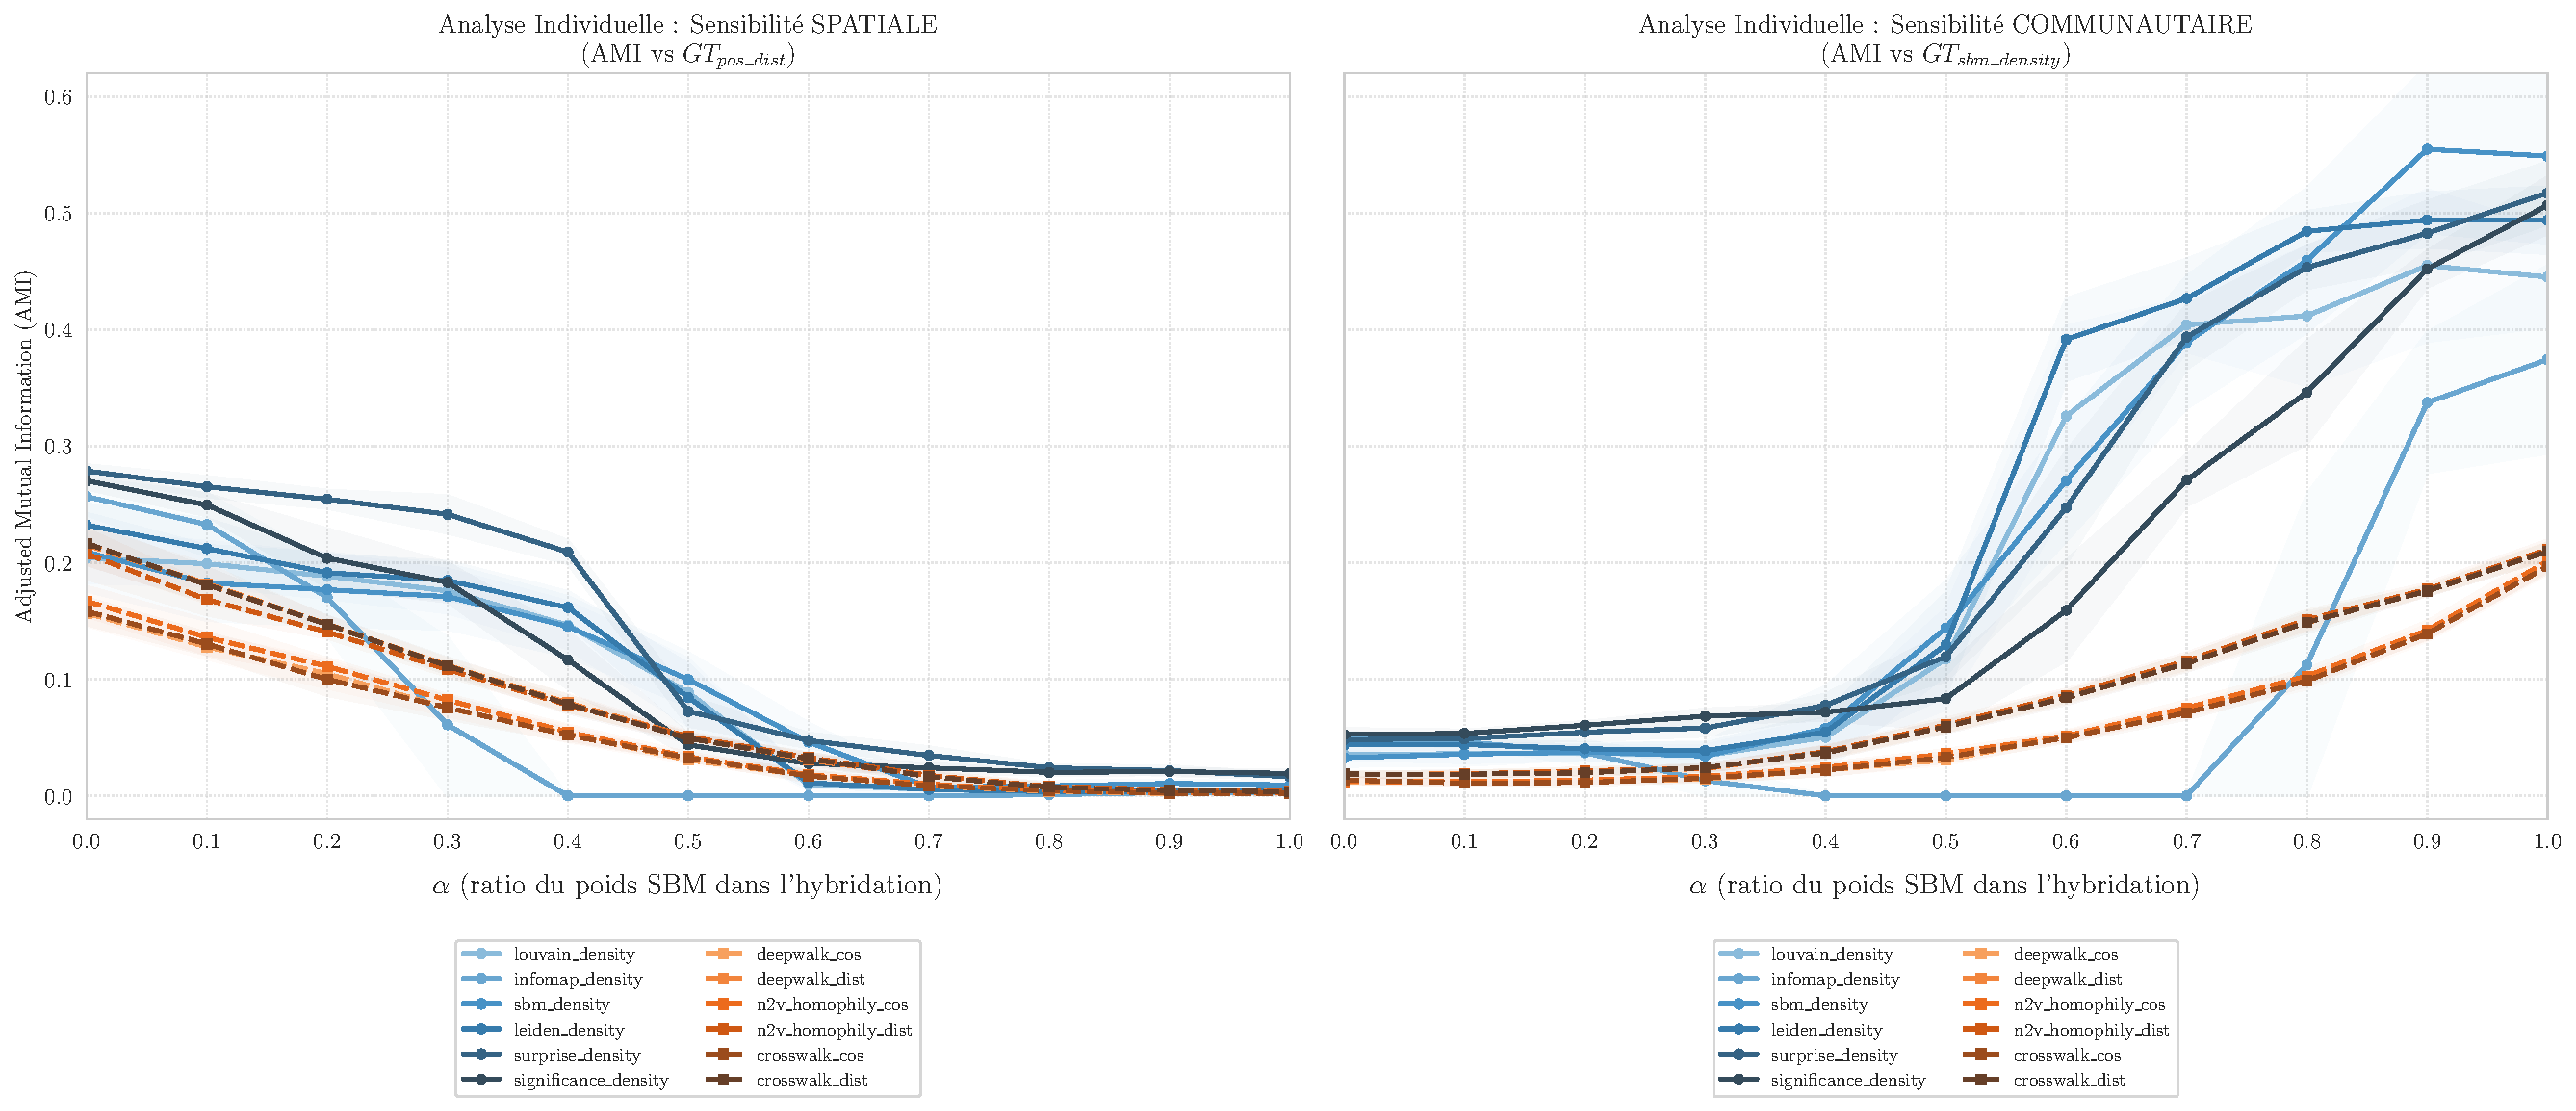
\includegraphics[width=\textwidth]{Plots/205 00_AMI_individual_features_VS_GT_comparison.pdf}
\caption{Evolution de l'Information Mutuelle Ajustée (AMI) entre les features et la \textit{Ground Truth} communautaire (à droite), et la \textit{Ground Truth} géométrique (à gauche) en fonction de $\alpha$ (moyenne sur 10 itérations).} \label{fig4}
\end{figure}


\subsection{Annexe 69 : Tables et graphes alternatifs mis de côté au cas où : }

\subsubsection{Table alternative à graph 1 SHAPvals GT\_pos et GT\_sbm pour validation}

\begin{table}[!ht]
\centering
\caption{Évolution des contributions SHAP globales moyennes de la \textit{Ground Truth} en fonction du ratio d'hybridation $\alpha$ (sur 10 expérimentations)}
\label{tab:validation_gt_shap}
\begin{tabular}{ccc}
\hline
\textbf{Ratio SBM ($\alpha$)} & \textbf{Contribution $\Phi_{\text{GT\_pos}}$} & \textbf{Contribution $\Phi_{\text{GT\_sbm}}$} \\
\hline
0.0 & 2,1644 $\pm$ 0,1245 & 0,2317 $\pm$ 0,0206 \\
0.1 & 1,8726 $\pm$ 0,0900 & 0,4158 $\pm$ 0,0533 \\
0.2 & 1,5545 $\pm$ 0,0554 & 0,5908 $\pm$ 0,0587 \\
0.3 & 1,3979 $\pm$ 0,0637 & 0,7387 $\pm$ 0,0348 \\
0.4 & 1,1828 $\pm$ 0,0692 & 0,8812 $\pm$ 0,0493 \\
0.5 & 1,1123 $\pm$ 0,0846 & 1,0491 $\pm$ 0,0498 \\
0.6 & 0,9279 $\pm$ 0,0564 & 1,1443 $\pm$ 0,0700 \\
0.7 & 0,8374 $\pm$ 0,0492 & 1,3730 $\pm$ 0,0538 \\
0.8 & 0,6641 $\pm$ 0,0530 & 1,5164 $\pm$ 0,0708 \\
0.9 & 0,4696 $\pm$ 0,0311 & 1,7690 $\pm$ 0,0415 \\
1.0 & 0,3167 $\pm$ 0,0300 & 2,2268 $\pm$ 0,1050 \\
\hline
\end{tabular}
\end{table}

\end{document}
